% This is a copy version from https://github.com/thanhhungqb/thesis-template
% * <thanhhungqb@gmail.com> 2017-05-09T23:23:15.758Z:
%
% ^.
% Please do not modified this project, when you want to start writing, make a clone of it for your own (Please read README.md)

\documentclass[12pt,a4paper,oneside]{book} % twoside for draf

% \usepackage{babel}
% \usepackage[utf8]{vietnam}
\usepackage[english,spanish]{babel}
\usepackage[utf8]{inputenc}
\usepackage{float}
%\usepackage{times}
%\usepackage{graphicx}

\usepackage{mathptmx}	% same Time New Roma
%\renewcommand{\rmdefault}{phv} % Arial
%\renewcommand{\sfdefault}{phv} % Arial

\usepackage{fancyhdr}
\usepackage{array}
\usepackage{amsmath,tabu}
\usepackage{makecell}
\usepackage{url}
\usepackage{algorithm2e}
\usepackage{parskip}
\usepackage{fancyhdr}

% \usepackage{subcaption}
\usepackage{subfigure}
\usepackage{graphicx}
\usepackage{caption}
\usepackage{lipsum}
\usepackage[pdftex,pdfpagelabels,bookmarks,hyperindex,hyperfigures]{hyperref}


%prevent to break long word
\tolerance=1
\emergencystretch=\maxdimen
\hyphenpenalty=10000
\hbadness=10000

\usepackage{titlesec, blindtext, color}
\definecolor{gray75}{gray}{0.75}
\newcommand{\hsp}{\hspace{20pt}}
\titleformat{\chapter}[hang]{\Huge\bfseries}{\thechapter{.}\hsp}{0pt}{\Huge\bfseries}

\usepackage{bkthesis}

\crname{LUẬN VĂN TỐT NGHIỆP}
\ctname{XÂY DỰNG MÔ HÌNH GAN\\TỪ ẢNH CHỤP CẮT LỚP VI TÍNH CT}
\cstuname{SVTH: }

\csCouncil{Khoa học máy tính}
\csSupervise{}
\csReviewer{}
\cttime{6/2019}


\thesislayout

\begin{document}
%-	Bìa cứng - màu xanh dương, chữ mạ vàng (xem mẫu đính kèm)
%-	Trang tên (tờ lót): chất liệu giấy, nội dung giống như bìa LV
%-	Ở gáy LV: in nhan đề LV (có thể in tóm tắt nếu nhan đề quá dài), size 15 – 17
%-	Phiếu Nhiệm vụ LV, chấm điểm Hướng dẫn & Phản biện (đã ký): nhận từ GVHD & GVPB sau khi bảo vệ (theo lịch hẹn).
%-	Lời cam đoan
%-	Lời cảm ơn/ Lời ngỏ
%-	Tóm tắt LV
%-	Mục lục
%-	Danh mục, bảng biểu, hình ảnh, ... (nếu có)
%-	Nội dung LV
%-	Danh mục TL tham khảo
%-	Phụ lục (nếu có)

\coverpage

\frontmatter

\chapter*{Lời cam đoan}
\noindent 
Đưa tiến bộ khoa học kỹ thuật vào ứng dụng thực tế trong đời sống là một nhu cầu thiết yếu và luôn được 
% Khai phá dữ liệu không phải là một đề tài mới nhưng vẫn luôn là một thách thức khó khăn bởi nguồn dữ liệu đầu vào rất đa dạng, phong phú và kết quả đầu ra phải đạt được những ý nghĩa nhất định. Trong quá trình nghiên cứu đề tài có rất nhiều kiến thức không nằm trong chương trình giảng dạy ở bậc Đại học tuy vậy chúng tôi xin cam đoan đây là công trình nghiên cứu của riêng chúng tôi dưới sự hướng dẫn của tiến sĩ Phan Trọng Nhân. Nội dung nghiên cứu và các kết quả đều là trung thực và chưa từng được công bố trước đây. Các số liệu được sử dụng cho quá trình phân tích, nhận xét được chính chúng tôi thu thập từ nhiều nguồn khác nhau và sẽ được ghi rõ trong phần tài liệu tham khảo. \\


Ngoài ra, chúng tôi cũng có sử dụng một số nhận xét, đánh giá và số liệu của các tác giả khác, cơ quan tổ chức khác. Tất cả đều có trích dẫn và chú thích nguồn gốc. \\

Nếu phát hiện có bất kì sự gian lận nào, chúng tôi xin hoàn toàn chịu trách nhiệm về nội dung đề cương luận văn của mình. Trường đại học Bách Khoa thành phố Hồ Chí Minh không liên quan đến những vi phạm tác quyền, bản quyền do chúng tôi gây ra trong quá trình thực hiện.
\begin{flushright}
Sinh viên thực hiện
\end{flushright}
\chapter*{Lời cảm ơn}
\noindent 	Để hoàn thành kì đề cương luận văn này, chúng tôi tỏ lòng biết ơn sâu sắc đến tiến sĩ Phan Trọng Nhân đã hướng dẫn tận tình trong suốt quá trình nghiên cứu. \\
	
Chúng tôi chân thành cám ơn quý thầy, cô trong khoa Khoa Học Và Kỹ Thuật Máy Tính, trường Đại học Bách Khoa thành phố Hồ Chí Minh đã tận tình truyền đạt kiến thức trong những năm chúng tôi học tập ở trường. Với vốn kiến thức tích lũy được trong suốt quá trình học tập không chỉ là nền tảng cho quá trình nghiên cứu mà còn là hành trang để bước vào đời một cách tự tin. \\
	
Cuối cùng, chúng tôi xin chúc quý thầy cô dồi dào sức khỏe và thành công trong sự nghiệp cao quý.
\begin{flushright}
Sinh viên thực hiện
\end{flushright}
	
\tableofcontents
% \listofsymbols
\listoftables
\listoffigures
% \listofalgorithms


\mainmatter

\fancyhead{}  % Clears all page headers and footers
%\rhead{\thepage}  % Sets the right side header to show the page number
%\lhead{}  % Clears the left side page header
%\fancyfoot[positions]{footer}
\renewcommand{\footrulewidth}{0.4pt}

\pagestyle{fancy}  % Finally, use the "fancy" page style to implement the FancyHdr headers

\chapter{Giới thiệu đề tài}
\section{Đặt vấn đề}
Trong y khoa, trực quan hoá dữ liệu là một nhu cầu thiết thực để tăng độ chính xác trong chuẩn đoán và điều trị nhiều loại tổn thương khác nhau của bệnh nhân. Đặc biệt đối với những loại chấn thương và bệnh lý ở các cơ quan nội tạng nằm bên trong cơ thể khi mà những bộ phận này không thể được quan sát trực tiếp bằng mắt thường, việc mô phỏng lại cơ quan đó thông qua các thiết bị kỹ thuật càng trở nên thiết yếu hơn. \\
Trước đây, phương pháp chụp X-quang cho phép hiển thị được hình chiếu của các bộ phận bên trong cơ thể nhờ vào mức độ hấp thụ khác nhau của các loại mô đối với tia X. Về sau, nhờ ứng dụng nhiều công nghệ kỹ thuật tiên tiến, người ta đã có thể chụp được nhiều ảnh X-quang từ nhiều hướng khác nhau rồi từ đó sử dụng các thiết bị vi tính để tính toán ra các ảnh cắt lớp của một vùng bất kỳ trên cơ thể bệnh nhân, kỹ thuật chụp ảnh này chính là Computed Tomography (CT).\\
Mặc dù đã đạt được một bước tiến đáng kể để có thể tái tạo được những hình ảnh các cơ quan nội tạng của bệnh nhân mà không cần mổ, song muốn có được một cái nhìn tổng thể ba chiều của một cơ quan bất kỳ vẫn cần sự can thiệp lớn của các bác sĩ. Hình khối ba chiều của một cơ quan nội tạng được xây dựng từ các ảnh cắt lớp của riêng bộ phận đó. Để có được ảnh cắt lớp riêng của một bộ phận từ ảnh CT cần các bác sĩ thực hiện nhận diện và phân đoạn chính xác bộ phận đó trên từng lát cắt của ảnh. Thông thường một ảnh CT ba chiều sẽ có số lát cắt từ một trăm đến bai trăm, mộ số ảnh chi tiết hơn có thể lên tới chín trăm lát cắt. Phải tiến hành phân đoạn trên một ảnh có nhiều lát cắt là thách thức lớn nhất của các bác sĩ khi muốn trực quan hoá một cơ quan nằm bên trong cơ thể lên không gian ba chiều.\\
Để giải quyết vấn đề về phân đoạn số lát cắt ba chiều lớn, nhiều giải pháp phân đoạn tự động đã được nghiên cứu và sử dụng. Tuy nhiên độ chính xác của các phương pháp này không cao do độ tương phản của các cơ quan rất giống nhau, đặc biệt là ở lồng ngực. Các phương pháp đạt hiệu quả cao hiện tại thường là các giải pháp bán tự động và cần sự can thiệp của đôị ngũ y bác sĩ.
\section{Mục tiêu đề tài}
Trong luận văn tốt nghiệp này, chúng tôi sẽ xây dựng một giải pháp phân đoạn tự động trên cơ sở của mạng học sâu để có thể trích xuất được thông tin bề mặt và trực quan hoá ba chiều cơ quan nội tạng từ ảnh CT chứa cơ quan đó. Để đánh giá giải pháp được xây dựng ở đề tài này, chúng tôi sẽ tiến hành so sánh mô hình của chúng tôi với các mô hình khác đã được các Luận văn tốt nghiệp trước trình bày. Bên cạnh đó chúng tôi cũng sẽ sử dụng các công cụ và tập dữ liệu đã được công khai có tính khách quan cao để đánh giá kết quả của mô hình được phát triển trong đề tài này. Và cuối cùng, chúng tôi sẽ xây dựng một ứng dụng cho phép phân đoạn tự động lá gan từ ảnh CT được người dùng đưa vào và hiển thị mô hình ba chiều cùng với ước lượng thể tích của lá gan đó.

\begin{figure*}
  \centering
  \subfigure[Ảnh CT lồng ngực]{%
    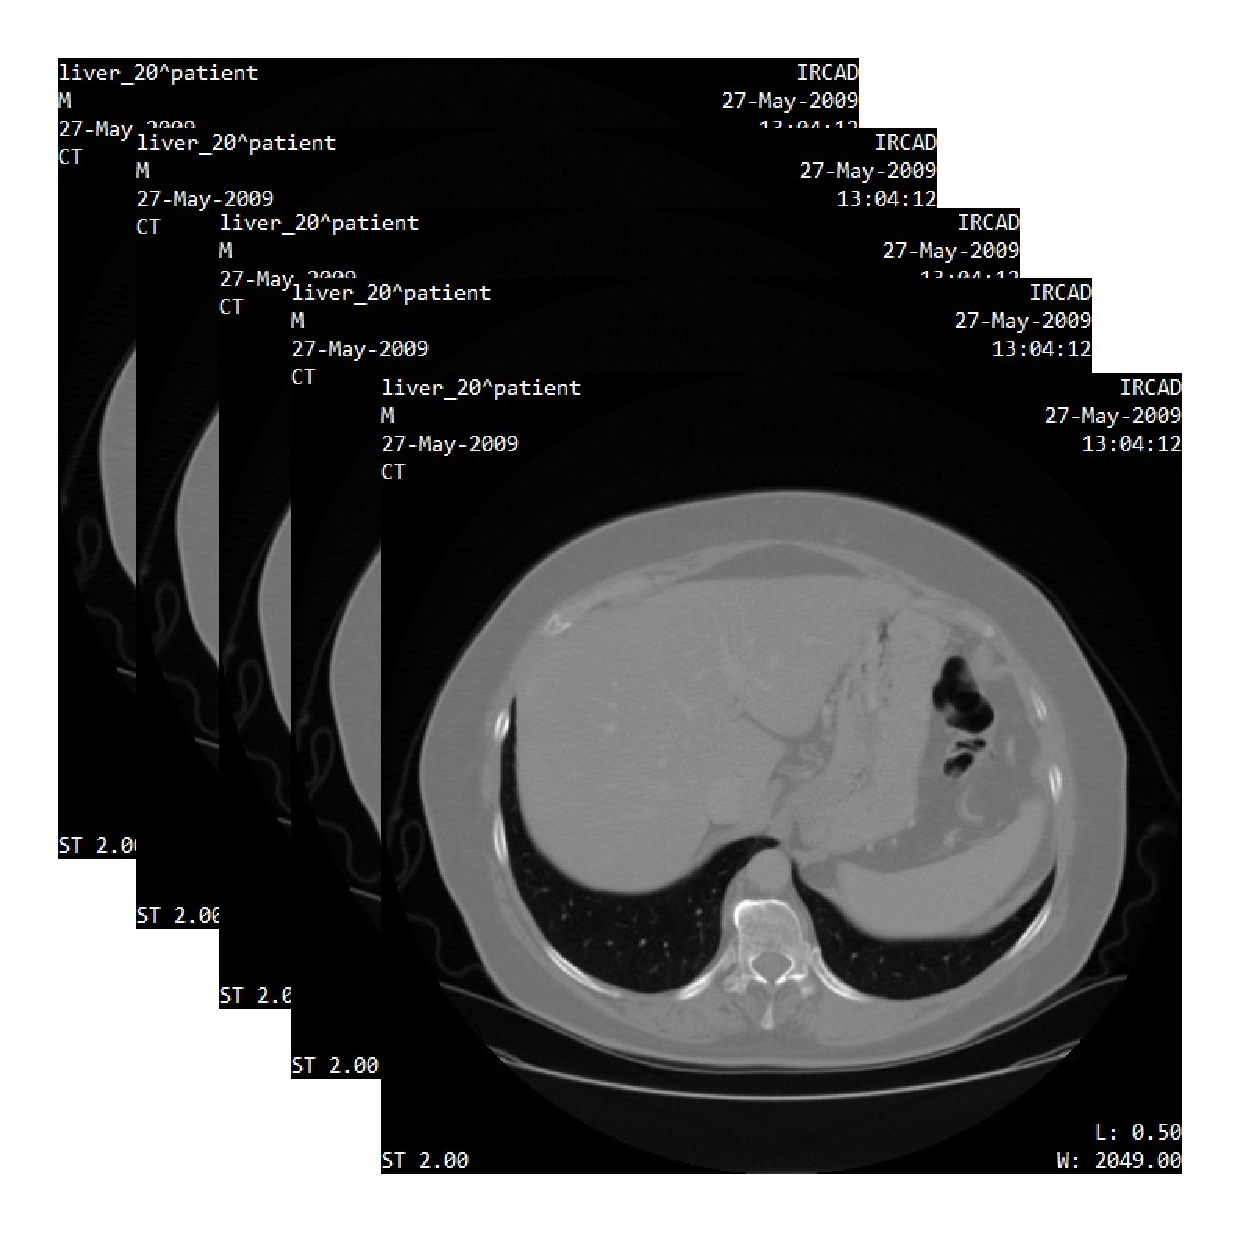
\includegraphics[width=0.3\textwidth]{Images/image5.pdf}%
    \label{fig:image5}%
    }
    \subfigure[Ảnh phân đoạn lá gan]{%
    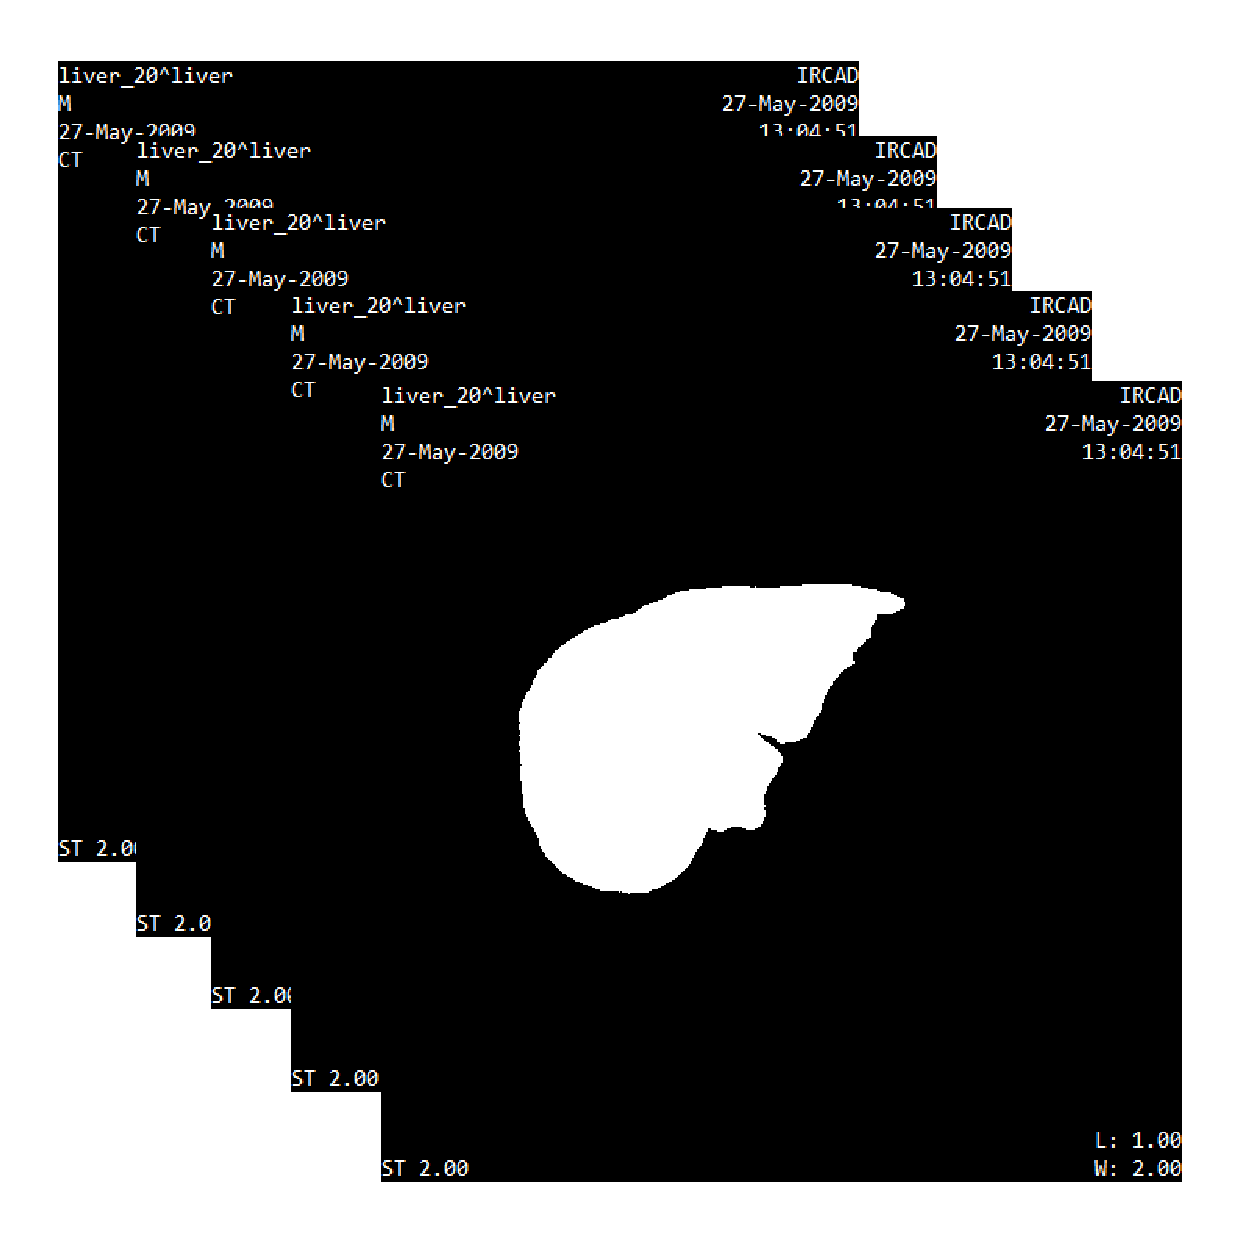
\includegraphics[width=0.3\textwidth]{Images/label5.pdf}%
    \label{fig:b}%
    }
    \subfigure[Ảnh lá gan 3 chiều]{%
    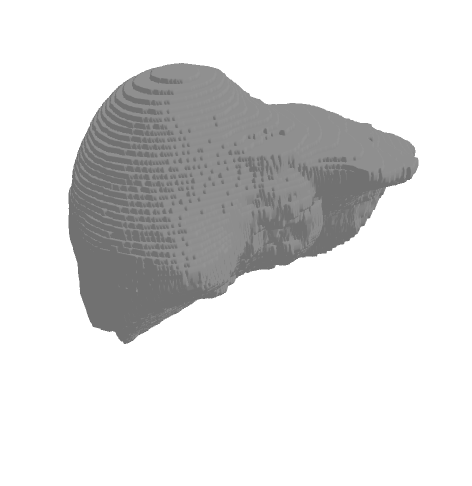
\includegraphics[width=0.3\textwidth]{Images/liver3d.png}%
    \label{fig:c}%
    }% 
  \caption{Minh hoạ quá trình xây dựng lá gan 3 chiều từ ảnh CT lồng ngực}
  \label{fig:ab}
\end{figure*}
\section{Phạm vi thực hiện}
Trong khuôn khổ của một Luận văn tốt nghiệp, chúng tôi sẽ giới hạn lại phạm vi nghiên cứu phù hợp để có thể đảm bảo được tính ứng dụng của đề tài và tính khách quan khi đánh giá mô hình được xây dựng với các mô hình khác. Ở đề tài này, chúng tôi sẽ tập trung vào xây dựng mô hình lá gan từ ảnh CT chụp lồng ngực bằng phương pháp chính là học sâu. Mô hình của chúng tôi sẽ được đánh giá với mô hình hai mô hình của anh Đàm Vũ Duy và của nhóm hai anh Bùi Hồng Thiên Nhật - Phạm Huỳnh Sơn. Giải pháp của chúng tôi cũng sẽ được đánh giá với các tập dữ liệu đã được sử dụng tại các hội nghị về xử lý ảnh y khoa có uy tín cáo SLiver07 \cite{website:slvier07}, 3Dircadb \cite{website:data_3DIRCADb}, LiTS2017 \cite{website:LiTS}.
\chapter{Trình tự công việc và bố cục luận văn}
\section{Trình tự công việc}
Để đạt được mục tiêu đề tài đặt ra, chúng tôi lần lượt tiến hành những công việc sau
\begin{enumerate}
    \item Khảo sát các tập dữ liệu sử dụng.
    \item Khảo sát các phương pháp xử lý ảnh giành cho kiểu dữ liệu vừa khảo sát.
    \item Khảo sát phương án và kết quả khi ứng dụng mạng học sâu vào xử lý ảnh y khoa.
    \item Tập trung nghiên cứu các mô hình học sâu có thể ứng dụng cho đề tài.
    \item Tiến hành xây dựng và thử nghiệm các mô hình học sâu trên các tập dữ liệu được công khai.
    \item Áp dụng một số kỹ thuật hậu xử lý phân đoạn để được kết quả chính xác hơn.
    \item Đánh giá các kết quả trên hệ thống Sliver07 và với phương pháp trong các luận văn trước.
    \item Đóng gói mô hình và xây dựng ứng dụng hiển thị.
\end{enumerate}
\section{Bố cục luận văn}
Luận văn này được trình bày thành 10 mục sắp xếp dựa trên trình tự thực hiện công việc của chúng tôi gồm:
\begin{enumerate}
    \item Giới thiệu đề tài
    \item Trình tự công việc và bố cục báo cáo
    \item Cơ sở lý thuyết
    \item Các mô hình tham khảo
    \item Khảo sát dữ liệu và tiền xử lý dữ liệu
    \item Huấn luyện, cải tiến và kiểm thử mô hình
    \item Hậu xử lý kết quả
    \item Đánh giá kết quả
    \item Xây dựng ứng dụng hiển thị
    \item Tổng kết
\end{enumerate}
\chapter{Cơ sở lý thuyết}
\section{Ảnh kỹ thuật số}
Ảnh kỹ thuật số là ảnh ở định dạng có thể lưu trữ trong và truyền tải qua các thiết bị điện tử. Hiện tại có hai loại định dạng cho ảnh kỹ thuật số là raster và vector. Ảnh raster được tạo thành từ các điểm ảnh được gọi là pixel. Ảnh vector được biểu diễn bằng các phép toán để tạo ra các đường nét trong ảnh. Trong luận văn này khi đề cập đến khái niệm ảnh hoặc ảnh kỹ thuật số nếu không nói gì thêm thì mặc định đó là ảnh raster.\\
Với ảnh kỹ thuật số, mỗi điểm ảnh sẽ được lưu bằng một hoặc nhiều giá trị nguyên, số giá trị nguyên đó được gọi là số kênh. Tuỳ vào từng định dạng ảnh khác nhau mà số kếnh và khoảng giá trị của mỗi kênh sẽ khác nhau.\\
Các ảnh CT y khoa tuân theo chuẩn DICOM (Digital Image and Communications in Medicine) thông thường sẽ có một kênh và được biểu thị bằng số nguyên 16-bit và được tổ chức xếp nhiều ảnh với nhau thành ảnh 3-chiều. Lúc này điểm ảnh pixel trên không gian hai chiều sẽ trở thành điểm ảnh voxel trên không gian ba chiều. Ảnh CT 3-chiều này sẽ đi kèm theo các thông tin về khoảng cách thực tế giữa hai voxel gần nhau trong không gian ba chiều. Nhờ đó ta có thể tính được diện tích và thể tích của vật thể nhờ vào số voxel của ảnh đó.

\section{Phân đoạn ảnh và các kỹ thuật phân đoạn cơ bản}
Trong bộ môn Thị giác máy tính, khái niệm phân đoạn ảnh được dùng để chỉ quá trình phân tách ảnh thành những tập hợp các pixel. Mục đích của quá trình này để giản lược hoặc thay đổi cách hiển thị ảnh có ý nghĩa và dễ để phân tích hơn. Một cách hiểu khác, phân đoạn ảnh là quá trình đánh nhãn cho từng pixel ảnh sao cho những pixel có cùng nhãn sẽ có cùng một số tính chất.\\
Khi ta thực hiện phân đoạn ảnh trên một chồng các ảnh của cùng vật thể theo đúng thứ tự, ví dụ như ảnh CT, kết quả của các phép phân đoạn này có thể dùng để tạo ra hình khối 3-chiều với các giải thuật như Marching cubes.\\
Một số kỹ thuật phân đoạn ảnh cơ bản có thể kể đến như:
\begin{itemize}
\item Phân đoạn ảnh theo ngưỡng: Phương pháp này khá đơn giản, nó chủ yếu dựa vào mức độ xám của các vùng trên ảnh để phân đoạn. Giải thuật thường được sử dụng là phương sai giữa các lớp lớn nhất(Otsu).
\item Phân đoạn dựa trên miền đồng nhất: Các miền trong ảnh sẽ dựa vào các tính chất (các tính chất sẽ có những giá trị khoảng về mức xám, màu sắc...) để phân đoạn. Từ ý tưởng này thì chúng ta có các cách sử dụng cho phương pháp này như tách cây tứ phân, cục bộ, tổng hợp…
\item Phân đoạn dựa vào biên của các đối tượng: Dựa trên một số giải thuật phát hiện biên như Sobel, Laplacian,... Những giải thuật này sẽ tìm được biên của một số đối tượng dựa trên các đặc điểm về chênh lệch màu sắc, mức xám trên ảnh. Từ đó chúng ta có thể phân đoạn được ảnh theo biên.
\end{itemize}
\textbf{Nhận xét:} Những phương pháp này có thể gọi là những phương pháp cổ điển để phân đoạn ảnh. Đặc điểm chung của nó là việc thực hiện nhanh chỉ qua vài phép toán biến đổi. Còn nhược điểm là bị sai nhiều khi các đối tượng trên ảnh không có sự khác nhau rõ ràng về màu sắc, mức xám. Việc sử dụng các phương pháp này chỉ để nghiên cứu và đánh giá hoặc công cụ hỗ trợ còn để ứng dụng vào thực tế thì vẫn rất hạn chế vì với các bài toán phức tạp thì các phương pháp này không thể đáp ứng được. Chúng ta có thể tìm hiểu thêm về các phương pháp này tại đây.\cite{segoverview}\\
Phương pháp tốt nhất hiện nay áp dụng cho các bài toán phân đoạn ảnh phức tạp là mạng học sâu. Tuy rằng chi phí để hiện thực và chạy mạng học sâu rất cao nhưng với các công cụ hỗ trợ hiện nay kết hợp với việc tận dụng được hiệu năng của GPU của mạng học sâu thì ngày nay nó được sử dụng rất nhiều và mang lại những kết quả vượt ngoài sức mong đợi. Và để giải thích cho điều này thì bên dưới sẽ trình bày chi tiết về mạng học sâu bao gồm cơ sở lý thuyết, trình bày và đánh giá một số mô hình trong mạng học sâu và một số kết quả mà nhóm đã làm được khi sử dụng nó.

\section{Lịch sử và những kiến thức cơ bản về mạng học sâu}
Phần này chúng tôi sẽ trình bày lại quá trình phát triển của mạng nơ-ron học sâu và phần nào lý giải nguyên do cho sự bùng nổ ứng dụng của mạng nơ-ron trong thời điểm hiện tại. Nội dung được chúng tôi tham khảo tại \cite{basicdeep}.\\
Trước hết chúng tôi nhắc lại các khái niệm như trí tuệ nhân tạo(Artificial Intelligence), học máy (Machine Learning) và học sâu(Deep Learning) viết tắt lần lượt là AI, ML và DL.
\begin{itemize}
    \item Khi máy tính có khả năng thực hiện những việc mà có đặc trưng như trí thông minh con người thì ta có thể gọi đó là trí tuệ nhân tạo.
    \item Khi máy tính có khả năng học từ dữ liệu được lưu trữ mà không phải lập trình một cách cụ thể thì đó là học máy.
    \item Học sâu là một trong những phương pháp của học máy sử dụng các mô hình mạng nơ-ron, ý tưởng chính dựa theo kiến trúc nơ-ron trong bộ não sinh học và các kết nối giữa chúng.
\end{itemize}
 Ta minh họa ba khái niệm này trong Hình \ref{history}.

\begin{figure}[ht]
\centering
        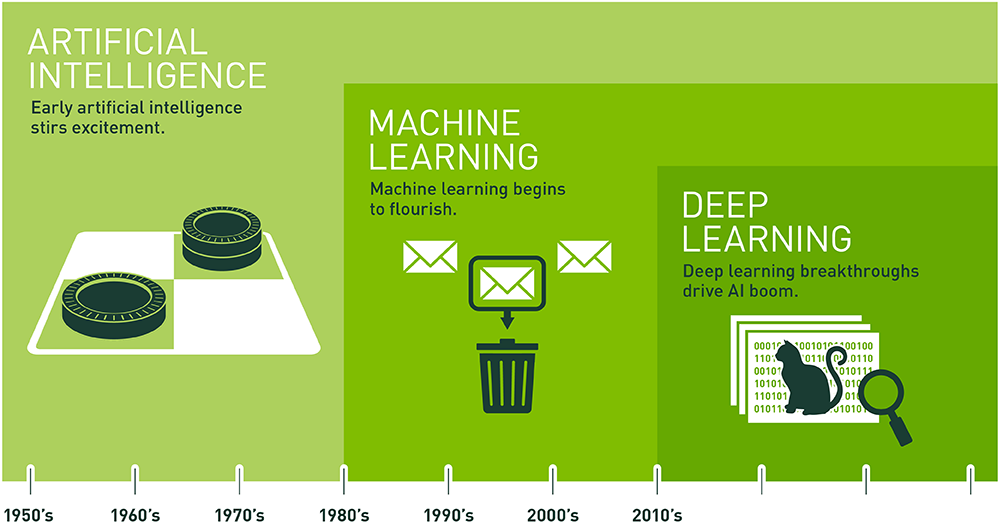
\includegraphics[totalheight=8cm]{Images/history.png}
    \caption{Minh họa AI, ML và DL\cite{basicai}}
    \label{history}
\end{figure}

\subsection{Giải thuật Perceptron Learning Algorithm(PLA)}
\begin{itemize}
\item PLA là nền móng đầu tiên của DL, nó được ra đời vào năm 1957 bởi Frank Rosenblatt giải bài toán về phân lớp nhị phân. Vì nó là nền móng nên hiểu được cách hoạt động của giải thuật này sẽ hiểu được cơ bản về DL. Vì sau này khi phát triển lên người ta chỉ cả tiến nó chứ không phải thay thế.
\item Yêu cầu của bài toán đặt ra là tìm phương trình một đường thẳng phân hai lớp đã được gán nhãn nằm về hai phía của đường thẳng đó, gọi là class 1 và class 2. Ý tưởng cơ bản của PLA là dự đoán, xây hàm mất mát, dựa vào hàm mất mát để đánh giá dự đoán và cập nhật lại dự đoán mới khi nào tốt thì dừng lại.
\item Trong không gian n chiều gọi \textbf{x} = [$x_{1}$, $x_{2}$, ..., $x_{n}$] là tập hợp các điểm dữ liệu, mỗi điểm được biểu diễn bằng một vector n chiều. \textbf{y} = [$y_{1}$, $y_{2}$, ..., $y_{n}$] là nhãn tức là giá trị lớp của mỗi điểm trong \textbf{x} tương ứng, $y_{i}$ = 1 nếu $x_{i}$ thuộc class 1, $y_{i}$ = -1 nếu $x_{i}$ thuộc class 2.
\item Ta giả sử đường thẳng cần tìm có phương trình:\[f_{x}(x) = w_{1}x_{1}+...+w_{n}x_{n}+w_{0}=w^{T}x = 0\]
Công việc của chúng ta là đi tìm các giá trị $w_{i}$ này hay còn gọi là các trọng số (weights).
\item Để dễ hình dung khi đi vào tính toán, ta sẽ đi tiếp trong trường hợp là không gian hai chiều (các công thức vẫn viết tổng quát cho n chiều). Ta giả sử đường thẳng $w_{1}$$x_{1}$ + $w_{2}$$x_{2}$ + $w_{0}$ = 0 là nghiệm của bài toán. Khi đó với điểm x chưa có nhãn, ta có thể gán nhãn cho nó bằng cách  \[label(x) = 1 \quad if \quad w^T \geq 0, \quad else \quad -1\] hay ngắn gọn là label(x) = sgn($w^{T}x$) với sgn là hàm xác định dấu.
\item Hàm mất mát này tính dựa trên số điểm bị phân lớp sai. Với mỗi điểm phân lớp sai thì y và $w^{T}$$x_{i}$ trái dấu, và khi phân lớp sai khoảng cách của điểm đó càng lớn thì giá trị hàm lỗi càng tăng. Việc chúng ta cần làm là đi tối ưu hàm lỗi này từ đó cập nhật được trọng số $w$. Ở đây sẽ đề xuất một phương pháp tối ưu áp dụng Gradient Descent đó là xét mỗi điểm bị phân lớp sai, khi đó giá trị mất mát cho điểm đó là: \[J(w; x_i; y_i) = -y_i w^T x_i\] có đạo hàm là $\Delta _{w}$J(w; $x_{i}$; $y_{i}$) = -$y_{i}$$x_{i}$.
\item Ta có quy tắc cập nhật là: $w_{t+1}^{T}$$x_{i}$ = ($w_{t}+y_{i} x_{i} )^{T}$$x_{i}$ =  $w_{t}^{T}$$x_{i}$ + $y_{i}$ $\left \| x_i \right \| ^{2}$.
Nhận thấy khi $w_{t}^T$$x_{i}$ và $y_{i}$ trái dấu, khi cập nhật lại thì $w_{t+1}^Tx_{i}$ < $w_{t}x_{i}$ nên hàm lỗi sẽ nhỏ đi theo mỗi bước cập nhật. Kết quả cuối cùng sẽ tối ưu nếu tập input có dạng tuyến tính. Mô hình minh họa cho PLA như Hình \ref{pla}. 
\end{itemize}

\begin{figure}[ht]
\centering
        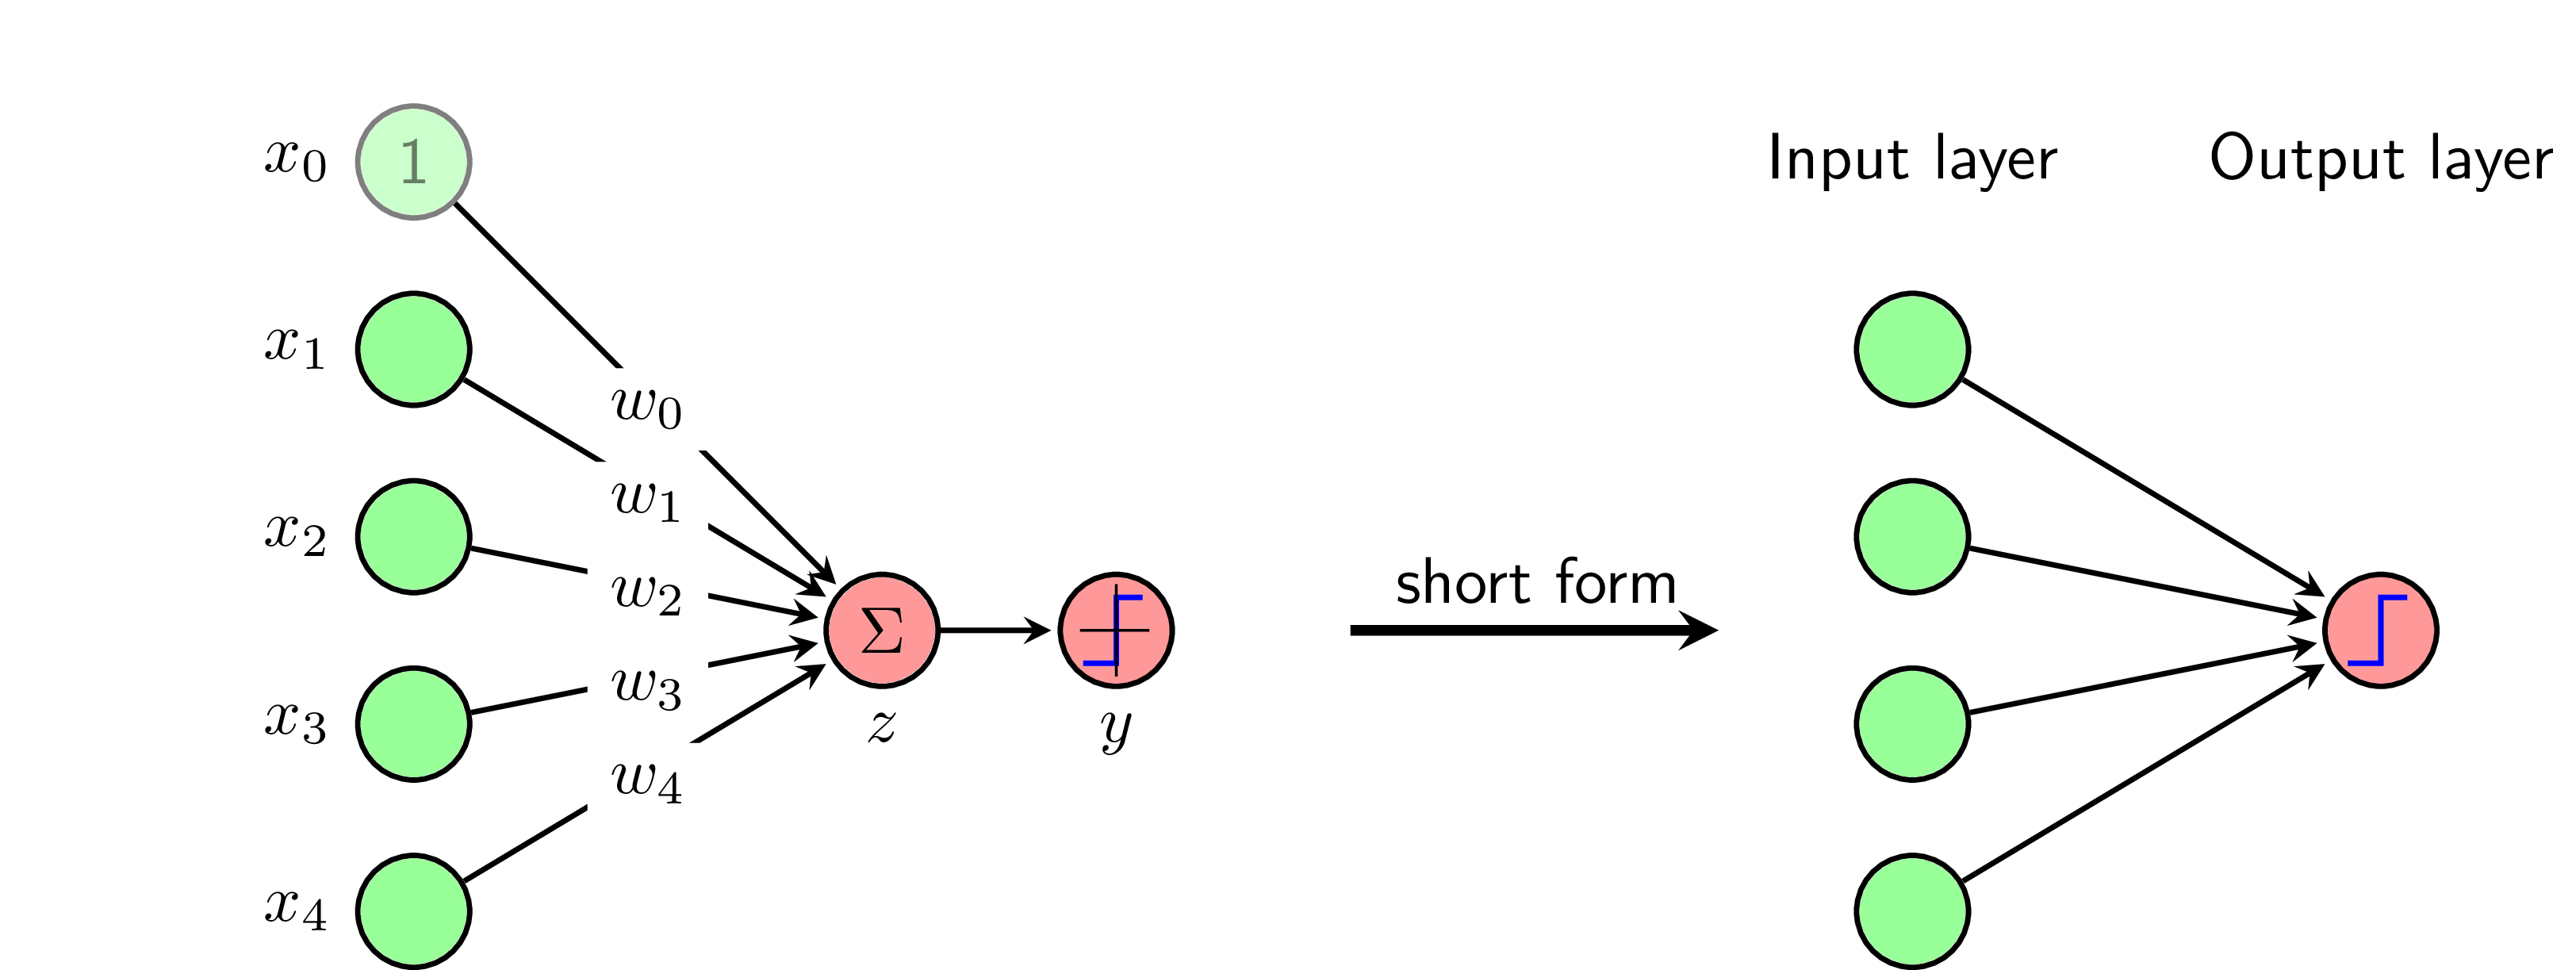
\includegraphics[totalheight=5cm]{Images/first_ann.png}
    \caption{Mô hình nơ-ron cho PLA \cite{basicdeep}}
    \label{pla}
\end{figure}

\begin{itemize}
\item Qua đây ta có thể giải thích được một số thành phần cơ bản trong một mạng nơ-ron. Lớp input là các giá trị $x$, các giá trị $w$ là các trọng số(weights), giá trị $x_{0}$=1 sau này sẽ được gọi là bias.
\item Với $z = w^{T}x$, ta có $y=sgn(z)$ là output của mạng. Hàm $sgn()$ được gọi là activation function.
Còn hàm lỗi thì chúng ta tự xây dựng và tự tối ưu miễn sao giải thuật có hiệu quả.
\end{itemize}
\subsection{MLP và Backpropagaion}
\begin{itemize}
\item Mặc dù PLA mang lại nhiều triển vọng lúc mới ra đời nhưng về bản chất thì nó không thể giải quyết được với tập dữ liệu phi tuyến và nó được chứng minh trong cuốn sách Perceptrons, điều này làm cho giải thuật này không phát triển được thêm trong hai mươi năm. Thời kỳ này còn được gọi là mùa đông AI thứ nhất(The first AI winter).
\item Mãi tới năm 1986, Geoffrey Hinton cùng cộng sự viết một bài báo có tên Learning representations by back propagating error chứng minh được rằng mạng nơ-ron với nhiều lớp ở giữa(gọi là hidden layer) có thể biểu diễn được các quan hệ phi tuyến với quy trình gọi là backpropagation và sau mỗi lớp là một hàm kích hoạt phi tuyến sigmoid hoặc tanh. Lúc này nó được gọi là Multi-layer Perceptron(MLP).
\item MLP cải tiến thêm chỗ thay vì chỉ có hai lớp input và output như PLA thì nó sẽ có thêm nhiều hidden layer ở giữa. Mỗi node ở các lớp này gọi là một Unit, input của mỗi Unit sẽ là output của lớp trước đó qua activation function. Giá trị $z$ ở mỗi Unit sẽ cộng thêm một giá trị $b$ được gọi là bias. Với MLP thì giá trị $b$ này không cố định là $1$ mà nó sẽ thay đổi trong quá trình học, qua các lớp, trên từng Unit.
\item Backpropagation là một phương pháp sử dụng để tối ưu hàm lỗi cho MLP, nó giúp tính gradient ngược từ lớp cuối cùng đến lớp đầu tiên dựa vào cách tính đạo hàm của hàm hợp. Nhờ đây mà mạng nơ-ron tiếp tục được phát triển cho tới khoảng 1990 do gặp phải vấn đề tiếp theo.
\end{itemize}
\subsection{Mùa đông AI thứ hai và sự ra đời của mạng học sâu}
\begin{itemize}
\item Vấn đề phi tuyến đã được giải quyết nhưng việc tối ưu hàm lỗi của mạng nơ-ron quá phức tạp khi gặp bài toán khó và dữ liệu đầu vào lớn vì nó không phải là một hàm lồi. Tiếp đến là việc các hidden layer mở rộng làm cho khả năng tính toán mất quá nhiều chi phí, làm cho việc huấn luyện không hiệu quả, và hơn nữa là vấn đề vanishing gradient (gradient bỏ qua những thành phần có đạo hàm =0). Những hạn chế này làm cho mạng nơ-ron bị thay thế dần bởi một giải thuật mới có tên là Support Vector Machine(SVM) trong giai đoạn 1990-2000. Giai đoạn này còn gọi là Mùa đông AI thứ hai.
\item Tới 2006, mạng nơ-ron được cải tiến bởi Hinton với khái niệm autoencoder. Ta có thể hiểu khái niệm nay bằng cách xây dựng nó như sau. Xây dựng một autoencoder là xây dựng một mạng nơ-ron chỉ có một hidden layer, số Unit của hidden layer này ít hơn số input và output thì bằng với input. Ta sẽ huấn luyện mạng này sao cho giá trị output giống với giá trị input. Vì mạng chỉ có một hidden layer nên ta có thể gọi giai đoạn từ input tới hidden layer là mã hóa, còn từ hidden layer tới output là giải mã. Quá trình này thành công, ta sẽ bỏ đi output vì về bản chất thì hidden layer tuy ít node hơn nhưng vẫn mang đầy đủ tính chất của input. Ta tiếp tục xây dựng một autoencoder từ hidden layer này và cứ thế cho đến khi đạt được một mạng đủ sâu mà output của mạng này mang được những đặc điểm của input. Sau đó ta tiếp tục làm việc với output này theo yêu cầu bài toán. Việc này sẽ làm giảm thiếu rất nhiều vấn đề vanishing gradient. Từ ý tưởng này, mạng nơ-ron được cộng đồng tiếp tục đón nhận và cũng kể từ đây cái tên mạng học sâu(Deep Learning) ra đời.
\item Năm 2012 là năm có nhiều biến động nhất, cũng kể từ đây mà DL chiếm ưu thế vượt trội hoàn toàn so với các phương pháp khác trong cùng lĩnh vực. Đầu tiên là việc ra đời của ReLU và dropout do Geoffrey Hinton và cộng sự công bố, hai kỹ thuật này khá đơn giản nhưng lại đem lại kết quả ngoài sức mong đợi. ReLU là hàm với output là 1 khi đầu vào không âm, là 0 khi ngược lại, còn dropout là trong quá trình huấn luyện một số hidden unit bị tắt ngẫu nhiên và khi test thì sẽ kích hoạt lại toàn bộ. Những phương pháp này mang lại nhiều hiệu quả và giảm thiểu được vanishing gradient. Tiếp đến là việc tận dụng được hiệu năng của GPU trong quá trình huấn luyện (GPU là card đồ họa với mục đích chính sản xuất là để chơi game với khả năng chạy song song nhiều lõi nhưng lại rất thích hợp khi huấn luyện các mạng học sâu, làm cho việc huấn luyện nhanh hơn rất nhiều lần).
\item Từ đó tới nay, mạng học sâu được sử dụng một cách rộng rãi hơn, các sản phẩm sử dụng nó, các nhà nghiên cứu, người học đều tăng cao, đồng thời các công cụ hỗ trợ việc code và huấn luyện cũng tăng lên nhanh chóng.
\end{itemize}

\section{Mạng nơ-ron học sâu tích chập và ứng dụng cho phân đoạn ảnh}
Các mạng nơ-ron truyền thống có thể giải những bài toán phức tạp với độ chính xác khá cao nhưng vấn đề chi phí đôi khi lại làm cho nó trở nên không khả thi. Đặc biệt sử dụng nó trong lĩnh vực xử lý ảnh. Ta lấy ví dụ một ảnh đầu vào có kích thước dài 128, rộng là 128 , ba giá trị màu là RGB sẽ có tới 128x128x3 = 49125 tham số cho mỗi lớp mạng để xử lý bức ảnh này. Hơn nữa các mạng nơ-ron phức tạp còn mắc phải vấn đề overfitting. Để giải quyết vấn đề này mạng nơ-ron tích chập (Convolutional Neural Networks hay ngắn gọn là CNN) là một dạng cải tiến của mạng nơ-ron nhân tạo được sử dụng. Ta sẽ đi vào phân tích một số đặc điểm của CNN để hiểu về rõ về cách giải quyết vấn đề của thiết kế mạng này.

% Toàn bộ kiến trúc CNN được minh họa như Hình \ref{cnn}.

% \begin{figure}[ht]
% \centering
%         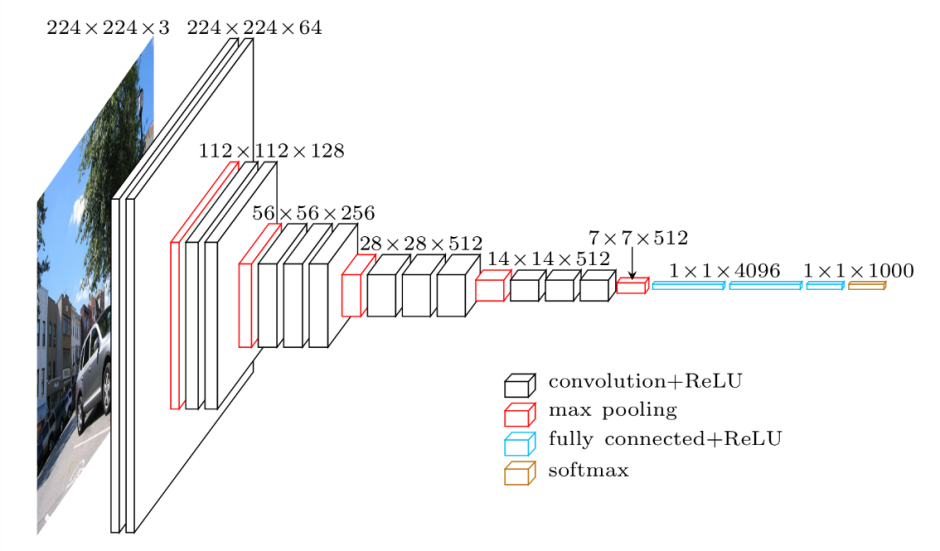
\includegraphics[totalheight=9cm]{Images/cnn.png}
%     \caption{Kiến trúc CNN\cite{accarchitect}}
%     \label{cnn}
% \end{figure}

\subsection{Lớp tích chập}
Trong xử lý ảnh và thị giác máy tính, người ta phân rõ hai khái niệm phép toán tích chập (convolution) và phép toán tương quan (correlation) qua điểm khác nhau duy nhất ở quá trình tính toán là đảo ngược ma trận lõi ở phép tích chập trước khi tính. Để dễ hình dung ta xem xét ví dụ sau đây với ma trận đầu vào 1-chiều $I$ (độ dài $i$) và lõi 1-chiều $K$ (độ dài $k$):
$$ I = [1, 2, 3, 4, 5, 6, 7, 8, 9]$$
$$ K = [2, 4, 6] $$
Thì kết quả của phép tính tương quan được tính như sau:
$$ Correlation(I,K)_{c = \overline{0, i - k - 1}} = \sum_{m=c}^{c + k-1}I_{m}*K_{m-c}$$
$$ Correlation(I,K) = [1*2 + 2*4 + 3*6, ... , 7*2 + 8*4 + 9*6] $$
$$ Correlation(I,K) = [28,  40,  52,  64,  76,  88, 100] $$
Và kết quả của phép tính tích chập được tính như sau:
$$ Convolution(I,K)_{c = \overline{0, i - k - 1}} = \sum_{m=c}^{c + k-1}I_{m}*K_{k - 1 - m + c}$$
$$ Convolution(I,K) = [1*6 + 2*4 + 3*2, ... , 7*6 + 8*4 + 9*2] $$
$$ Convolution(I,K) = [20, 32, 44, 56, 68, 80, 92] $$
Công thức trên tham khảo tại \cite{convSlide}. tương tự khi I, K là các ma trận 2, 3 chiều. Để dễ hình dung ta xem hình minh hoạ \ref{convExample}.

\begin{figure}[h]
\centering
    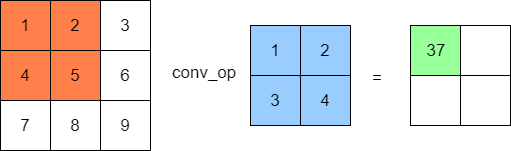
\includegraphics[totalheight=2.7cm]{Images/conv.png}
    \caption{Phép tính tương quan trong xử lý ảnh}
    \label{convExample}
\end{figure}
Ta có thể thấy ở phép tính tương quan trên ma trận, tuỳ vào ma trận lõi $K$ mà ma trận kết quả sẽ có được một số tính chất đặt biệt, ví dụ ở hình \ref{convExample} ta sẽ nhận được ma trận kết quả làm nổi bật các cạnh dọc ở ma trận đầu vào. Điều tương tự cũng xảy ra với kết quả của phép tính tích chập vì hai phép tính này là gần giống nhau ở cách tính. Trong các phép tính xử lý ảnh, tuỳ vào tình huống mà người ta sử dụng phép tích chập hoặc phép tính tương quan để nhầm đạt được độ lợi về thời gian tính toán khi tính áp dụng các tính chất kết hợp lên một dãy các phép tính tích chập (tương quan) liên tục\cite{convtheorem}.\\
Tuy nhiên ở các mạng học sâu, phép tính tích chập được dùng để chỉ phép tính tương quan. Các nên tảng học sâu được hỗ trợ như Tensorflow sử dụng từ khoá tích chập và lớp tích chập để chỉ phép tính tương quan trong xử lý ảnh. Vì như đã nói ý nghĩa của hai phép tính này là như nhau, tuỳ vào độ lợi tính toán mà người ta sẽ quyết định sử dụng phép tính nào.\\
Khi sử dụng lớp tích chập thay cho lớp kết nối đầy đủ ở mạng học sâu sẽ có một số khác biệt sau:
\begin{itemize}
    \item Bộ nhớ tính toán sử dụng các lớp tích chập sẽ nhỏ hơn.
    \item Thời gian tính toán khi sử dụng các lớp tích chập sẽ nhanh hơn.
    \item Ở những lớp càng sâu, một điểm dữ liệu khi sử dụng các lớp tích chập sẽ bị ảnh hưởng bới nhiều điểm dữ liệu đầu vào hơn thay vì là như nhau ở tất cả các lớp.
\end{itemize} 
Trong mạng học sâu, quá trình học sẽ giúp cập nhật các trọng số ở ma trận lõi $K$.

\subsection{Lớp gộp}
Lớp gộp (pooling), đôi khi được gọi là lớp giảm kích thước mẫu (sub-sampling), thường được sử dụng sau một số lớp tích chập nhất định. Ta có thể thấy sau khi qua một số lớp tích chập nhất định, ảnh thường sẽ có hiện tượng bị nhoè do những điểm ảnh gần nhau có giá trị gần giống nhau. Lớp gộp này đóng vai trò làm giảm kích thước ảnh nhưng vẫn đảm bảo giữ lại các dữ liệu cần thiết nhằm qua đó làm giảm số lượng phép tính toán và tránh tình trạng quá khớp (overfitting).\\
Lớp gộp có thể sử dụng nhiều loại hàm gộp khác nhau như hàm trung bình hoặc hàm lấy lớn nhất (phổ biến) tuỳ thuộc vào đặc điểm của bài toán. Các lớp gộp này thường có kích thước bằng với độ cách (stride), tức là chúng sẽ có ý nghĩa như một phép thay thế một vùng các điểm dữ liệu chỉ bằng một điểm dữ liệu duy nhất, và các vùng này không có điểm trùng.\\
Ta có thể thấy sau khi qua một lớp gộp, các vùng khác nhau sẽ nằm gần nhau hơn và nhờ vậy với lớp tính tích chập tiếp theo sẽ có được thông tin của một vùng lớn hơn ở ảnh ban đầu. Vì vậy sau khi qua càng nhiều lớp gộp, ảnh (đặc trưng) sẽ có ý nghĩa toàn cục hơn là ý nghĩa chi tiết. Đây cũng là một yếu điểm của lớp gộp cho bài toán phân đoạn ảnh mà không thay đổi kích thước của nó.

\begin{figure}[h]
\centering
    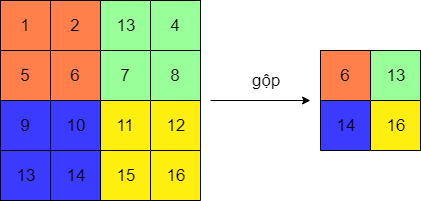
\includegraphics[totalheight=3.5cm]{Images/max-pool.png}
    \caption{Phép tính gộp lấy lớn nhất với kích thước 2, độ cách 2}
    \label{poolExample}
\end{figure}

\subsection{Lớp đảo tích chập}
Phép đảo tích chập, có tên gọi khác là phép chuyển vị (transpose), là phép tính ngược lại với phép tích chập. Ở phép đảo tích chập, mỗi giá trị trong ma trận ảnh gốc $S$ sẽ được nhân với một ma trận trọng số lõi $K$ để được một vùng giá trị của ảnh kết quả $R$, các vùng này có thể chồng lấn lên nhau tuỳ vào độ cách (stride) và kích thước của $K$. Trong xử lý ảnh, phép đảo tích chập thường được dùng để phóng to và làm rõ các loại ảnh như ảnh chụp kính hiển vi, ảnh nguyên tử, ảnh thiên văn...  Trong mạng học sâu, quá trình học sẽ giúp cập nhật các trọng số ở ma trận lõi $K$.

\begin{figure}[h]
\centering
    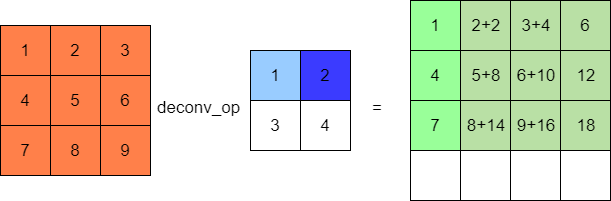
\includegraphics[totalheight=3.2cm]{Images/deconv.png}
    \caption{Phép tính đảo tích chập với kích thước 2, độ cách 1}
    \label{deconvExample}
\end{figure}

\begin{figure}[h]
\centering
    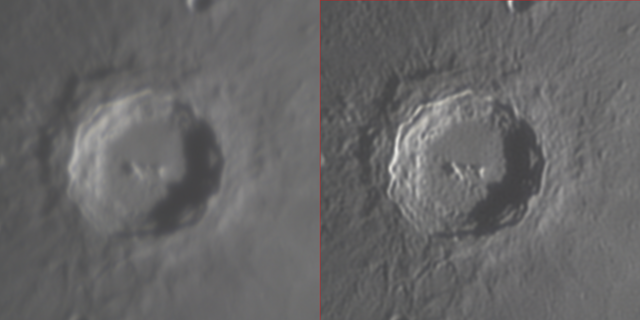
\includegraphics[totalheight=3.2cm]{Images/realConvEx.png}
    \caption{Ảnh chụp thiên văn trước và sau khi được xử lý đảo tích chập}
    \label{deconvRealExample}
\end{figure}


\section{Các chỉ số đánh giá kết quả phân đoạn}
Kết quả phân đoạn có thể được đánh giá bằng nhiều cách khác nhau. Đối với một bài toán nhất định, mỗi chỉ số đánh giá được lựa chọn cần phải nhạy cảm với một số đặc điểm phụ thuộc vào mục đích bài toán đó. Nếu bài toán để xác định thể tích vật thể, sai khác thể tích sẽ là chỉ số tiên quyết cho bài toán đó. Tuy nhiên với một kết quả phân đoạn cho ra thể tích chính xác hoàn toàn trên lý thuyết vẫn có thể bị sai hoàn toàn nếu như sử dụng chỉ số trùng giao trên hợp của voxel. Vì vậy, mỗi bài toán phải luôn dùng nhiều chỉ số phân đoạn khác nhau để đánh giá các giải pháp cho bài toán đó.\\
Trong luận văn này, chúng tôi sử dụng các chỉ số của cuộc thi phân đoạn lá gan trên tập dữ liệu SLiver07 tham khảo tại \cite{SLiver07metric}. Các chỉ số này sẽ được tính ra điểm cho từng chỉ số và cuối cùng tính trung bình ra tổng điểm cho một kết quả phân đoạn. Với mỗi chỉ số, mức điểm hoàn hảo là 100 điểm, mức điểm chấp nhận được là 75 điểm, mức điểm thấp nhất là 0 điểm. Mức điểm hoàn hảo là kết quả phân đoạn của chuyên gia đã có kinh nghiệm cho lĩnh vực phân đoạn bộ phận đó. Mức điểm chấp nhận được là của sinh viên y khoa chưa có kinh nghiệm phân đoạn khi so với kết quả của chuyên gia.\\
Các chỉ số được chúng tôi sử dụng bao gồm:
\begin{itemize}
    \item Chỉ số lỗi thể tích (Volumetric overlap error - VOE), giá trị phần trăm. Chỉ số này được tính như sau: lấy tổng số voxel giao giữa dự đoán và nhãn chia cho tổng số voxel hợp giữa dự đoán và nhãn, lấy 1 trừ kết quả đó rồi nhân cho 100.
    \item Chỉ số sai khác thể tích tuyệt đối (Relative absolute volume difference - VD), giá trị phần trăm. Chỉ số này được tính bằng hiệu số thể tích của phép phân đoạn và nhãn, chia cho nhãn, nhân 100. Chỉ số này nhận giá trị âm khi thể tích phân đoạn nhỏ hơn thể tích nhãn và nhận giá trị dương khi thể tích phân đoạn lớn hơn thể tích nhãn. Lưu ý chỉ số này có thể đạt điểm 100 khi kết quả phân đoạn không trùng với nhãn.
    \item Khoảng cách mặt đối xứng trung bình (Average symmetric surface distance - AvgD), giá trị milimet. Voxel cạnh của vật thể là voxel có ít nhất 1 trong 18 láng giềng không thuộc vật thể. Khoảng cách mỗi voxel tới bề mặt là khoảng cách ngắn nhất từ voxel đó đến một voxel thuộc bề mặt. Khoảng cách trung bình giữa hai bề mặt là giá trị trung bình của tất cả các voxel tới bề mặt kia (voxel thuộc dự đoán tới bề mặt nhãn, voxel thuộc nhãn tới bề mặt dự đoán).
    \item Khoảng cách mặt đối xứng bình phương từ gốc (Root Mean Square symmetric surface distance - RMSD), giá trị milimet. Giá trị này được tính giống với  AvgD nhưng khoảng cách ban đầu sẽ được bình phương lên và lấy trung bình.
    \item Khoảng cách mặt lớn nhất (Maximum symmetric surface distance - MaxD), giá trị milimet. Chỉ số này tính giống AD nhưng thay vì lưu trung bình sẽ lưu giá trị lớn nhất.
\end{itemize}
Lưu ý các chỉ số trên là các chỉ số lỗi, càng thấp tức là kết quả phân đoạn càng tốt. Điểm cho mỗi chỉ số sẽ bằng 100 trừ đi chỉ số nhân với một hệ số đã xác định, và lấy lớn hơn với 0. \\

\begin{table}
\begin{center}
\begin{tabular}{ |l|c| } 
\hline
\Gape[0.1cm][0.1cm]{Tên chỉ số} & Công thức chỉ số \\ 
\hline
\textbf{VOE} &\Gape[0.5cm][0.5cm]{$(1 - {R \bigcap G}/{R\bigcup G})*100\%$ }\\ 
\hline
\textbf{VD} & \Gape[0.5cm][0.5cm]{$(|R| -|G|)/|G|*100\%$} \\ 
\hline
\textbf{AvgD} & \Gape[0.5cm][0.5cm]{$(\sum d(S(G),S(R)) + \sum d(S(R),S(G)))/(|S| + |G|)$}\\
\hline
\textbf{RMSD} & \Gape[0.5cm][0.5cm]{$\sqrt{(\sum d(S(G),S(R))^{2} + \sum d(S(R),S(G))^{2})/(|S| + |G|)}$} \\ 
\hline
\textbf{MaxD} & \Gape[0.5cm][0.5cm]{$max(max(d(S(G),S(R))), max(d(S(G),S(R))))$} \\ 
\hline
\end{tabular}
\caption{\label{tab:table-name1}Cách tính các chỉ số.}
\end{center}
\end{table}


\begin{table}[H]
\begin{center}
\begin{tabular}{ |l|c| } 
\hline
\Gape[0.1cm][0.1cm]{Tên chỉ số} & Công thức điểm \\ 
\hline
\textbf{VOE} & \Gape[0.5cm][0.5cm]{$100 - 100*\textbf{VOE}*25/6.4$} \\ 
\hline
\textbf{VD} & \Gape[0.5cm][0.5cm]{$100 - 100*\textbf{|VD|}*25/4.7$} \\ 
\hline
\textbf{AvgD} & \Gape[0.5cm][0.5cm]{$100 - 100*\textbf{AvgD}*25$} \\
\hline
\textbf{RMSD} & \Gape[0.5cm][0.5cm]{$100 - 100*\textbf{RMSD}*25/1.8$} \\ 
\hline
\textbf{MaxD} &\Gape[0.5cm][0.5cm]{ $100 - 100*\textbf{MaxD}*25/4.7$} \\ 
\hline
\end{tabular}
\caption{\label{tab:table-name}Cách tính điểm cho các chỉ số.}
\end{center}
\end{table}
 
Ý nghĩa của các ký hiệu như sau:
\begin{itemize}
    \item $G$: vật thể nhãn
    \item $R$: vật thể được dựa đoán bởi mô hình
    \item $\bigcap$: phần thể tích giao của hai vật thể
    \item $\bigcup$: phần thể tích hợp của hai vật thể
    \item $|R|$: tổng số voxel của vật thể R
    \item $S(R)$: bề mặt vật thể R
    \item $d(x,S(R))$: khoảng cách từ voxel x đến bề mặt vật thể R
    \item $d(S(G),S(R))$: khoảng cách một chiều từ bề mặt vật thể G tới bề mặt vật thể R, đây là tập hợp $\{ d(v_{0}, S(R)), d(v_{1}, S(R)),...d(v_{n}, S(R)) \} $ với $v \in S(G) $
    \item $\textbf{|VD|}$: giá trị tuyệt đối của chỉ số VD.
\end{itemize}
\chapter{Các mô hình mạng tham khảo chính}
% \section{Định hướng phát triển mô hình}
\section{Mô hình mạng đảo tích chập cơ bản dùng cho phân đoạn ảnh}
Trong bối cảnh các mô hình mạng học sâu tích chập (Convolution neural networks - CNN) đã cho thấy khả năng phân loại ảnh vượt bậc, nhiều mô hình mới dựa trên kiến trúc này để giải quyết bài toán khác dần được phát triển và có được kết quả rất khả quan. Trong đó có thể đến như \cite{object_detection_ex1} và \cite{object_detection_ex2} để nhận diện vị trí vật thể, \cite{segmentation_ex1} và \cite{segmentation_ex2} để phân đoạn vật thể, \cite{action_recognize_ex1} để nhận diện hành vi người.\\
Trong đó, các mạng dùng để phân đoạn ảnh dựa trên CNN sẽ được chuyển về mạng tích chập đầy đủ (Fully Convolutional Network) bằng cách loại bỏ tất cả các lớp liên kết đầy đủ và thay thế bằng cách lớp tích chập. Các mạng FCN này sẽ gán nhẵn cho từng điểm ảnh và thực hiện một phép phóng to ảnh cơ bản bằng phương pháp nội suy. Một số công trình giới thiệu kết quả tốt hơn bằng việc sử dụng trường điều kiện ngẫu nhiên sau khi đã sử dụng mạng học sâu.\\
Các phương án phân đoạn ảnh vừa nêu đều có một số hạn chế nhất định. Khi sử dụng giải pháp phóng lớn ảnh bằng phương pháp nội suy điểm ảnh, ảnh kết quả thường bị thô và nhoè vì với phương pháp này giá trị điểm ảnh mới có độ chính xác không cao. Còn khi sử dụng trường điều kiện ngẫu nhiên để làm mượt ảnh, tốc độ rất hạn chế và đòi hỏi máy tính phải có cấu hình mạnh, đặc biệt khi sử dụng phương pháp này cho một ảnh 3-chiều. Để giải quyết các hạn chế đó, Hyeonwoo Noh và cộng sự giới thiệu mô hình mạng đảo tích chập \cite{unpoolref} theo thiết kế của một mạng tích chập đầy đủ (FCN).
\subsection{Kiến trúc mạng}
Mạng đảo tích chập của Hyeonwoo và cộng sự sử dụng kiến trúc mã hoá và giải mã quen thuộc của các mạng phân đoạn. Mô hình mạng này là một cải tiến của loại mạng VGG16 với các điểm đặc biệt sau:
\begin{itemize}
    \item Phần mã hoá sử dụng các khối mạng gồm các lớp tích chập và gộp có số lượng và cấu hình như mạng VGG16. 
    \item Loại bỏ các lớp kết nối đầy đủ ở VGG16, thay bằng các lớp tích chập. Phần mã hoá trở thành một phiên bản FCN của VGG16.
    \item Phần giải mã thiết kế đối xứng với phần mã hoá.
    \item Kích thước ảnh ở đầu vào và đầu ra của mạng là giống nhau.
\end{itemize}
\begin{figure}[h]
\centering
    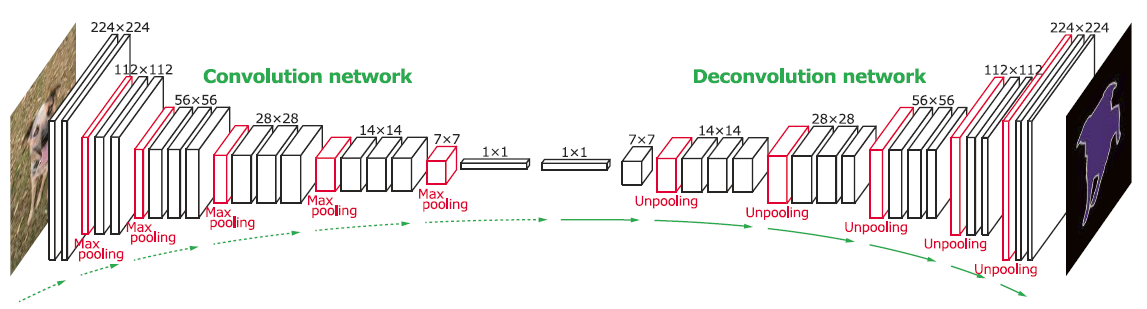
\includegraphics[totalheight=4cm]{Images/deconvNet.png}
    \caption{Mô hình mạng đảo tích chập của Hyeonwoo Noh và cộng sự}
    \label{deconvNet}
\end{figure}

\subsection{Các lớp mạng}
Trong \cite{unpoolref}, Hyeonwoo và cộng sự đã có một thay đổi nhỏ ở phần mã hoá so với VGG16 đó là sử dụng lớp chuẩn hoá (Batchnorm) để tránh tình trạng bão hoà gradient khiến mạng không thể được cập nhật trọng số. Các lớp chuẩn hoá này được thiết kế đặt sau mỗi lớp tích chập và lớp đảo tích chập. Theo các tác giả, lớp chuẩn hoá được thêm vào do chiều sâu của mạng đảo tích chập đã được tăng lên gấp đôi so với VGG16, thay đổi này nhằm tránh lại nhược điểm khó học của các mạng có độ sâu quá lớn.\\
Các lớp gộp được thiết kế để loại bớt giá trị nhiễu bằng cách sử dụng một giá trị đại diện cho một vùng ảnh. Mặc dù mang tính chất đại diện cho nhiều điểm ảnh, nhưng cách làm như vậy lại vô tình khiến mạng bị mất thông tin. Để giải quyết vấn đề này, mạng đảo tích chập sử dụng một bảng nhớ và dùng nó lại trong quá trình đảo gộp. Chi tiết xem tại mục phép đảo gộp trình bày ở chương Cơ sở lý thuyết.\\
Để xây dựng lại ảnh phân đoạn có kích thước ảnh gốc trong quá trình giải mã. Mạng đảo tích chập sử dụng phép đảo tích chập có kích thước và số các ma trận lõi gần như đối xứng với phần mã hoá. Tuy nhiên, số ma trận lõi của lớp tích chập ở trước mỗi lớp đảo gộp bị giảm đi một nửa so với các lớp tích chập khác trong khối mã hoá.\\
Tất cả các hàm kích hoạt được sử dụng là hàm Relu, trừ lớp đảo tích chập cuối cùng sử dụng hàm softmax để phù với mục đích phân đoạn của bài toán cho nhiều lớp đối tượng (class).
\subsection{Huấn luyện mạng}
Trong \cite{unpoolref}, mạng đảo tích chập được huấn luyện để sử dụng phân đoạn cho bộ dữ liệu PASCAL VOC 2012. Hyeonwoo và cộng sự sử dụng các trọng số trong phần mã hoá đã được huấn luyện cho mạng VGG16 với tập ILSVRC (pretrain). Quá trình huấn luyện sử dụng tốc độ học (learning rate) 0.01, đà (momentum) 0.9, khử trọng số (weight decay) 0.0005.

\section{Mô hình mạng đảo tích chập với phương pháp huấn luyện giám sát sâu (DSN)}
Trong bài toán phân đoạn ảnh, mạng nơ-ron tích chập với kiến trúc mã hóa, giải mã (encoder - decoder) là một trong những mô hình học sâu truyền thống được sử dụng rộng rãi nhất. Kỹ thuật huấn luyện mô hình này bằng phương pháp giám sát sâu đã được giới thiệu trong bài báo "3D Deeply Supervised Network for Automatic Liver Segmentation from CT Volumes" bởi Qi Dou và cộng sự\cite{dsn_paper}.
Khi huấn luyện mô hình (Train time), hai lớp giải mã tương ứng được thêm vào mạng tạo ra phần "Deep Supervision". Như vậy, mô hình lúc này sẽ có ba cổng ra và đồng thời cũng sẽ có ba hàm mất mát tương ứng với từng cổng ra. Hàm mất mát toàn phần lúc này là tổng hợp giữa hàm mất mát chính và các hàm mất mát phụ:\\
\begin{center} $Loss = \mu_1 Loss_{6} + \mu_2 Loss_{3} + \mu_3 Loss_{main}$\end{center}
\begin{figure}[h]
\centering
    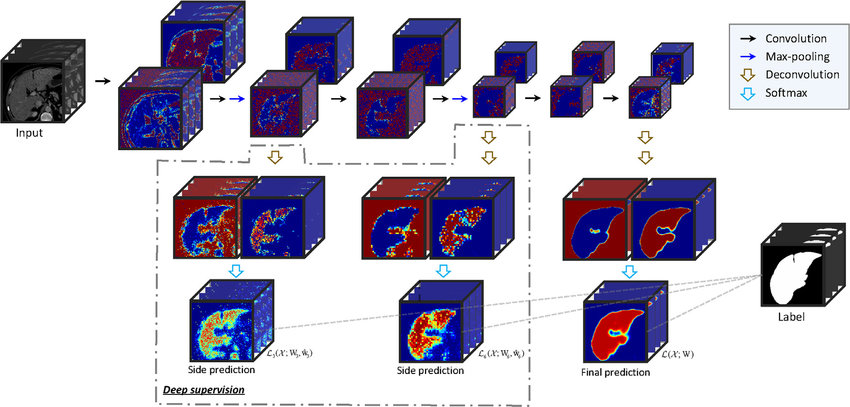
\includegraphics[totalheight=8cm]{Images/The-architecture-of-the-proposed-3D-DSN-taking-3D-liver-segmentation-as-an-example.png}
    \caption{Kiến trúc mô hình mạng đảo tích chập với phương pháp huấn luyện giám sát sâu (DSN)}
    \label{DSN}
\end{figure}
Với phương pháp huấn luyện mô hình này, trọng số trên phần mã hóa sẽ được cập nhật và chia sẽ giữa các luồng thay vì chỉ trên luồng chính. Việc này nhằm tăng khả năng học các đặc trưng quan trọng giúp phân đoạn chính xác lá gan, đồng thời giảm khả năng "vanishing gradient".
\section{Mô hình mạng Unet}
Mô hình mạng Unet được giới thiệu trong bài báo "U-Net: Convolutional Networks for Biomedical Image Segmentation" vào ngày 18 tháng 5 năm 2015 bởi Olaf và các cộng sự.\cite{unet_paper}\\
Mạng Unet là sự kết hợp của các lớp tích chập, lớp gộp, lớp gộp kênh và lớp phóng lớn kích thước mẫu (up-sampling). Tên mạng Unet được đặt theo kiến trúc giống hình chữ U của mạng với hai phần gần như đối xứng nhau. Mạng Unet có kiến trúc tương tự với các mạng sử dụng cho mục đích phân đoạn ảnh khác khi kiến trúc mạng có thể chia ra hai phần là mã hoá (encoder) và giải mã (decoder). Điểm khác biệt của mạng Unet là cách xử lý trong quá trình làm lơn kích thước mẫu khi sử dụng các kết nối tắt từ phần mã hoá đến phần giải mã. Qua đó kết quả phân đoạn được làm tốt hơn đáng kể. Phần sau đây sẽ trình bày lại các chi tiết hơn các đặc điểm mạng Unet của Olaf và các cộng sự. 
\subsection{Kiến trúc phần mã hoá}
Phần mã hoá của mạng sử dụng các lớp tích chập và lớp gộp như các mạng dùng cho xử lý ảnh khác. Tuy nhiên so với các mạng dùng cho xác định, phân loại ảnh như VGG16, VGG19, Resnet, thì Unet có độ sâu nhỏ hơn. Mạng Unet tô chức các lớp tích chập và gộp với nhau thành những khối mã hoá, mỗi khối gồm hai lớp tích chập và một lớp gộp sau cùng (trừ khối cuối cùng không có lớp gộp là là khối trung gian giữa giải mã và mã hoá). Tuỳ vào mục đích sử dụng và tình huống khác nhau, các siêu tham số của các lớp này sẽ được cấu hình khác nhau. Thông thường, các lớp này sử dụng các ma trận lõi có kích thước 3x3, số ma trận lõi mỗi lớp của khối sau sẽ gấp đôi khối trước, hàm kích hoạt là Relu, khối gộp sử dụng hàm lớn nhất với ma trận 2x2. Phần mã hoá này có tác dụng tìm ra các đặc điểm chung và phổ quát của ảnh đầu vào, chấp nhận mất mát thông tin trong quá trình.

\subsection{Kết nối tắt}
Ở mỗi khối mã hoá, trước khi ảnh được xử lý gộp sẽ có một kết nối để giữ những giá trị chưa gộp này và đưa chúng vào một khối giải mã. Kết nối đầy đủ này xuất hiện trước tất cả các lớp gộp. Như vậy, nhược điểm của các lớp gộp là làm mất thông tin giờ đã được khắc phục bằng các kết nối tắt, có tác dụng giữ lại tất cả các thông tin có thể mất mát do quá trình gộp để dùng cho quá trình giải mã, giúp cho ảnh phân đoạn cuối cùng trở nên chi tiết hơn.

\begin{figure}[h]
\centering
    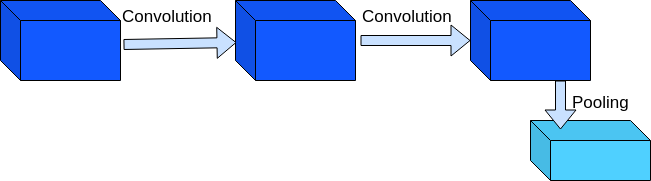
\includegraphics[totalheight=3cm]{Images/encoder_block.png}
    \caption{Dữ liệu được xử lý trong mỗi khối mã hoá}
    \label{skip_conn}
\end{figure}

\begin{figure}[h]
\centering
    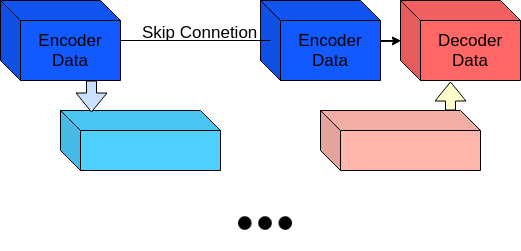
\includegraphics[totalheight=4.5cm]{Images/skip_conn.png}
    \caption{Dữ liệu truyền qua kết nối tắt}
    \label{skip_conn}
\end{figure}

\begin{figure}[h]
\centering
    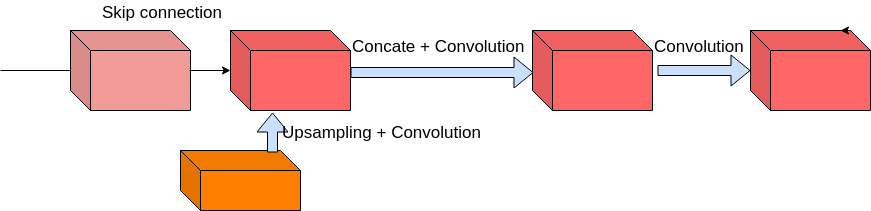
\includegraphics[totalheight=3.45cm]{Images/decoder_block.png}
    \caption{Dữ liệu được xử lý trong khối giải mã}
    \label{skip_conn}
\end{figure}

\subsection{Kiến trúc phần giải mã}
Phần mã hoá thông tin có tác dụng tìm ra những đặc điểm phổ quát của ảnh, còn phần giải mã có tác dụng tạo ra kết quả phân đoạn từ những thông tin đã được mã hoá. Phần giải mã được cấu tạo từ các lớp phóng lớn, lớp nối kênh và lớp tích chập thành các khối giải mã. Khối giải mã có cấu trúc gần đối xứng với khối mã hoá gồm lần lượt một khối tăng kích thước, một khối tích chập, một khối nối kênh, hai khối tích chập. Cấu hình siêu tham số các lớp giải mã giống với cấu hình siêu tham số các lớp ở quá trình mã hoá. Dữ liệu từ lớp trung gian khi đi qua từng khối giải mã sẽ được lớp phóng to làm lớn gấp đôi, các lớp tích chập sử dụng số ma trận lõi có kích thước 3x3, số ma trận lõi của lớp trước gấp đôi lớp sau, lớp cộng kênh được sử dụng cho kết quả lớp phóng lớn và dữ liệu của kết nối tắt.

\begin{figure}[h]
\centering
    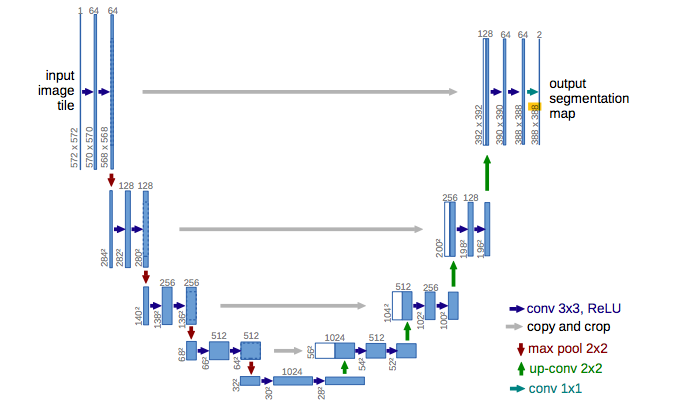
\includegraphics[totalheight=9.5cm]{Images/unet.png}
    \caption{Toàn bộ kiến trúc mạng Unet}
    \label{skip_conn}
\end{figure}

\subsection{Hàm lỗi}
Trong \cite{unet_paper}, Olaf và cộng sự sử dụng hàm lỗi cross-entropy. Tuy nhiên tuỳ vào đặc tính các tập dữ liệu khác nhau, mà nhiều hàm lỗi khác nhau có thể được sử dụng như hàm Dice, hàm cross-entropy với trọng số.

\subsection{Mạng Unet 3-chiều}
Trong \cite{3DUnet}, Ozgun Cikek và cộng sự đã giới thiệu một mô hình mạng Unet 3-chiều dùng cho xử lý các ảnh cắt lớp được tổ chức chung với nhau thành một khối và có thể coi như một ảnh 3-chiều, đây là định dạng của các ảnh CT và MRI.\\
So với mạng Unet, mạng Unet 3-chiều của Ozgun Cikek và cộng sự có một số điểm khác biệt sau:
\begin{itemize}
    \item Sử dụng ảnh đầu vào là các ảnh chụp lát cắt liên tục.
    \item Sử dụng các ma trận lõi 3-chiều, thực hiện phép tính tích chập, gộp, gộp kênh 3-chiều.
    \item Giảm số khối mã hoá và giải mã (từ 4 khối về 3 khối).
    \item Giảm số ma trận lõi ở mỗi lớp tích chập.
    \item Gấp đôi số kênh bằng cách gấp đôi số ma trận lõi trước khi thực hiện phép gộp (Unet của Olaf thực hiện sau) nhằm giảm thiểu sự mất mát dữ liệu.
    \item Sử dụng phép chuẩn hoá (batchnorm) sau các hàm kích hoạt.
\end{itemize}

\begin{figure}[h]
\centering
    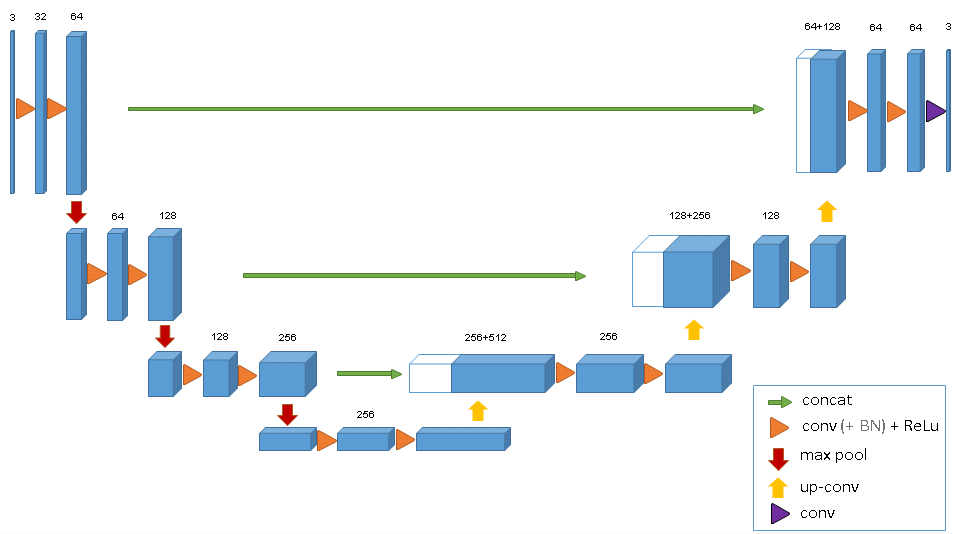
\includegraphics[totalheight=7cm]{Images/3Dunet.png}
    \caption{Kiến trúc mạng Unet 3-chiều}
    \label{skip_conn}
\end{figure}




\chapter{Khảo sát dữ liệu và tiền xử lý dữ liệu}
\section{Các tập dữ liệu sử dụng}
Để mô hình xây dựng đủ độ chính xác và có tính ứng dụng thực tế cũng như có thể được đánh giá khách quan, chúng tôi sử dụng các tập dữ liệu bệnh nhân thật đã được các y bác sĩ có chuyên môn tiến hành phân đoạn và công bố rộng rãi tại nhiều cuộc thi, hội nghị trên toàn thế giới. Cụ thể chúng tôi sử dụng các tập dữ liệu sau đây:
\begin{itemize}
    \item \textbf{SLiver07}: Đây là tập dữ liệu được sử dụng trong một cuộc thi thuộc khuôn khổ hội nghị MICCAI 2007 dành cho các hệ thống phân đoạn lá gan tự động và bán tự động.. Số mặt cắt trong tập ảnh nằm trong khoảng từ 64 đến 388 ảnh 2-chiều.  Khoảng cách mỗi điểm ảnh trong mỗi ảnh cắt ngang nằm trong khoảng 0.55 đến 0.8 mi-li-mét, khoảng cách hai mặt cắt liên tiếp từ 1 đến 3 mi-li-mét. Mỗi ảnh CT đều đi kèm với các thông số trên. Trong tập dữ liệu SLiver07 được công bố, chúng tôi sử dụng 20 ảnh CT có đánh nhãn cho quá trình huấn luyện và 10 ảnh CT không có nhãn cho hệ thống chấm điểm online tại \cite{website:slvier07}.
    \item \textbf{3DIRCADb-01}: Đây là tập dữ liệu của trường Đại học Bệnh viện IRCAD tại Pháp. Tập dữ liệu này gồm 20 ảnh CT lồng ngực của 20 bệnh nhân (10 nam - 10 nữ) và ảnh phân đoạn được thực hiện của các bác sĩ có chuyên môn của rất nhiều cơ quan trong lồng ngực gồm: phổi, gan, xương, động mạch, thận, khối u gan.... Số mặt cắt trong tập ảnh nằm trong khoảng từ 91 đến 260 ảnh 2-chiều. Các ảnh trong tập dữ liệu này có các khoảng cách giữa các điểm ảnh từ 0,56 đến 0,81 mi-li-mét, khoảng cách hai mặt cắt từ 1,6 đến 4 mi-li-mét. Tất cả ảnh trong tập dữ liệu này đều có đánh nhãn cho lá gan và được chúng tôi sử dụng làm tập huấn luyện cho mô hình.
    \item \textbf{LiTS}: Đây là tập dữ liệu được sử dụng trong cuộc thi tổ chức kết hợp với Hội nghị ISBI (thuộc IEEE) và MICCAI năm 2017 dành cho hệ thống phân đoạn lá gan và khối u gan. Tập dữ liệu là kết quả sự hợp tác của 7 bệnh viện và viện nghiên cứu. Số mặt cắt trong tập ảnh nằm trong khoảng từ 42 đến 1026 ảnh 2-chiều. Khoảng cách mỗi điểm ảnh trong mỗi ảnh cắt ngang nằm trong khoảng 0.65 đến 1.0 mi-li-mét, khoảng cách hai mặt cắt liên tiếp từ 0.45 đến 0.6 mi-li-mét. Tổng số ảnh của tập dữ liệu này là 201 ảnh CT, trong đó có 131 ảnh công bố có nhãn được chúng tôi sử dụng làm dữ liệu huấn luyện và 70 ảnh không có nhãn được chúng tôi sử dụng tạo kết quả kiểm tra và gửi cho hệ thống chấm tự động.
\end{itemize}
Ảnh CT 3-chiều trong các ảnh này là các ảnh CT 2-chiều xếp chồng lên nhau theo thứ tự và khoảng cách được ghi rõ cho từng ảnh. Các ảnh CT 2-chiều chụp mặt cắt ngang của cơ thể theo chiều dọc (mặt cắt song song với mặt đất khi người đứng thẳng) từ nhiều loại máy khác nhau và cũng được các chuyên gia phân đoạn theo góc nhìn này. Các ảnh CT được tạo thành từ nguyên lý giống với kỹ thuật chụp ảnh X-quang tức đo mức độ hấp thụ tia xạ khác nhau của các loại mô khác nhau. Các giá trị được lưu trong các tập dữ liệu này đều là các giá trị thể hiện mức độ hấp thu đó và vì vậy sẽ được chúng tôi xử lý phù hợp trước khi huấn luyện.

\section{Tiền xử lý dữ liệu}
\subsection{Chuẩn hóa dữ liệu}
\paragraph{Hounsfield unit (HU)} Hounsfield unit (còn được gọi là số CT), được đặt theo tên Sir Godfrey Hounsfield,là thang đo định lượng mô tả mật độ phóng xạ trong ảnh chụp cắt lớp vi tính. Giá trị HU của không khí được định nghĩa -1000 HU và của nước là 0 HU.
\paragraph{Chuẩn hóa giá trị Hounsfield unit (HU)} Bao gồm các bước sau:
\begin{enumerate}
\item Đưa thang đo về khoảng [-1000, 400]: Thay đổi giá trị HU của những voxel có giá trị thấp hơn -1000 HU về -1000 HU, những voxel có giá trị cao hơn 400 HU về 400 HU
\item Đưa thang đo về khoảng [0, 1400]: Cộng 1000 (HU) vào giá trị mỗi voxel
\item Chuẩn hóa giá trị [0,1]: Chia giá trị mỗi voxel cho 1400
\end{enumerate}
Sau bước chuẩn hóa, giá trị trên mỗi voxel nằm trong khoảng [0,1] dạng 32-bit single-precision floating-point.

\begin{figure*}
  \centering
  \subfigure[Chưa thực hiện tiền xử lý]{%
    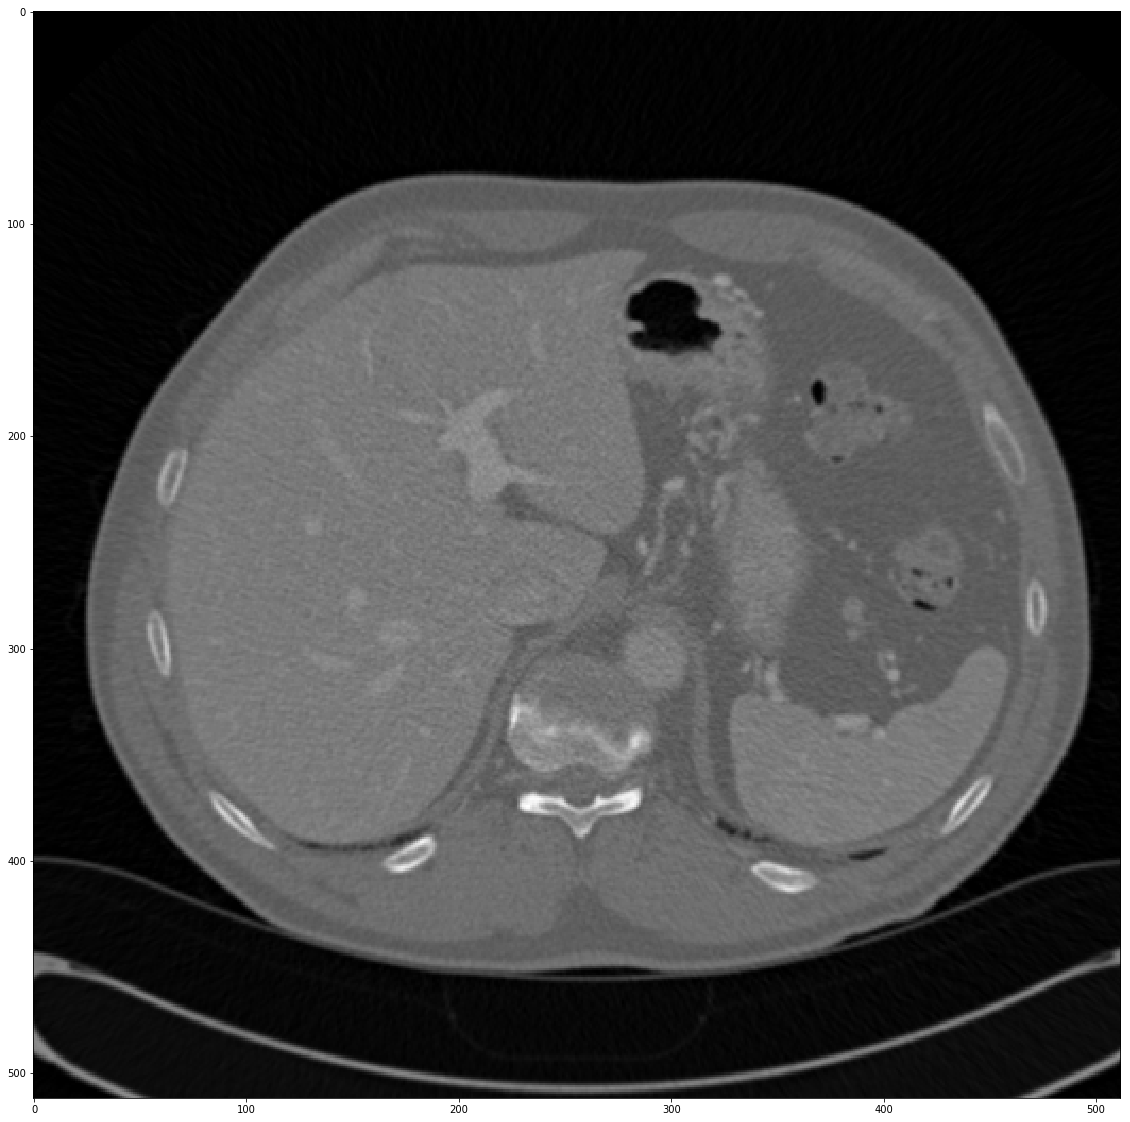
\includegraphics[width=0.3\textwidth]{Images/Liver_org.png}%
    \label{fig:image5}%
    }
    \subfigure[Sau khi chuẩn hóa.]{%
    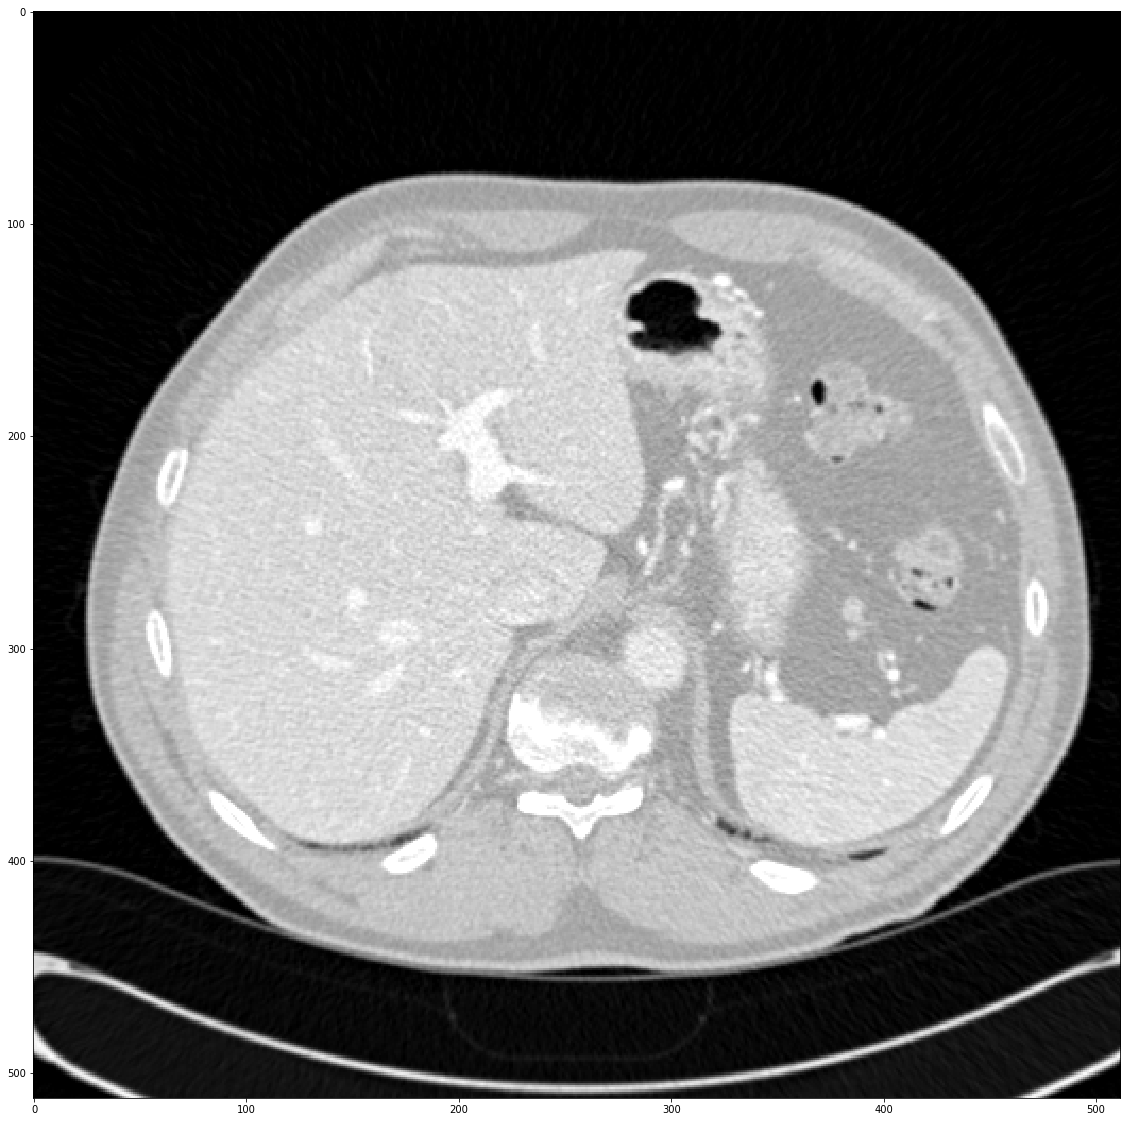
\includegraphics[width=0.3\textwidth]{Images/Liver_norm.png}%
    \label{fig:b}%
    }
    \subfigure[Đã loại bỏ nhiễu.]{%
    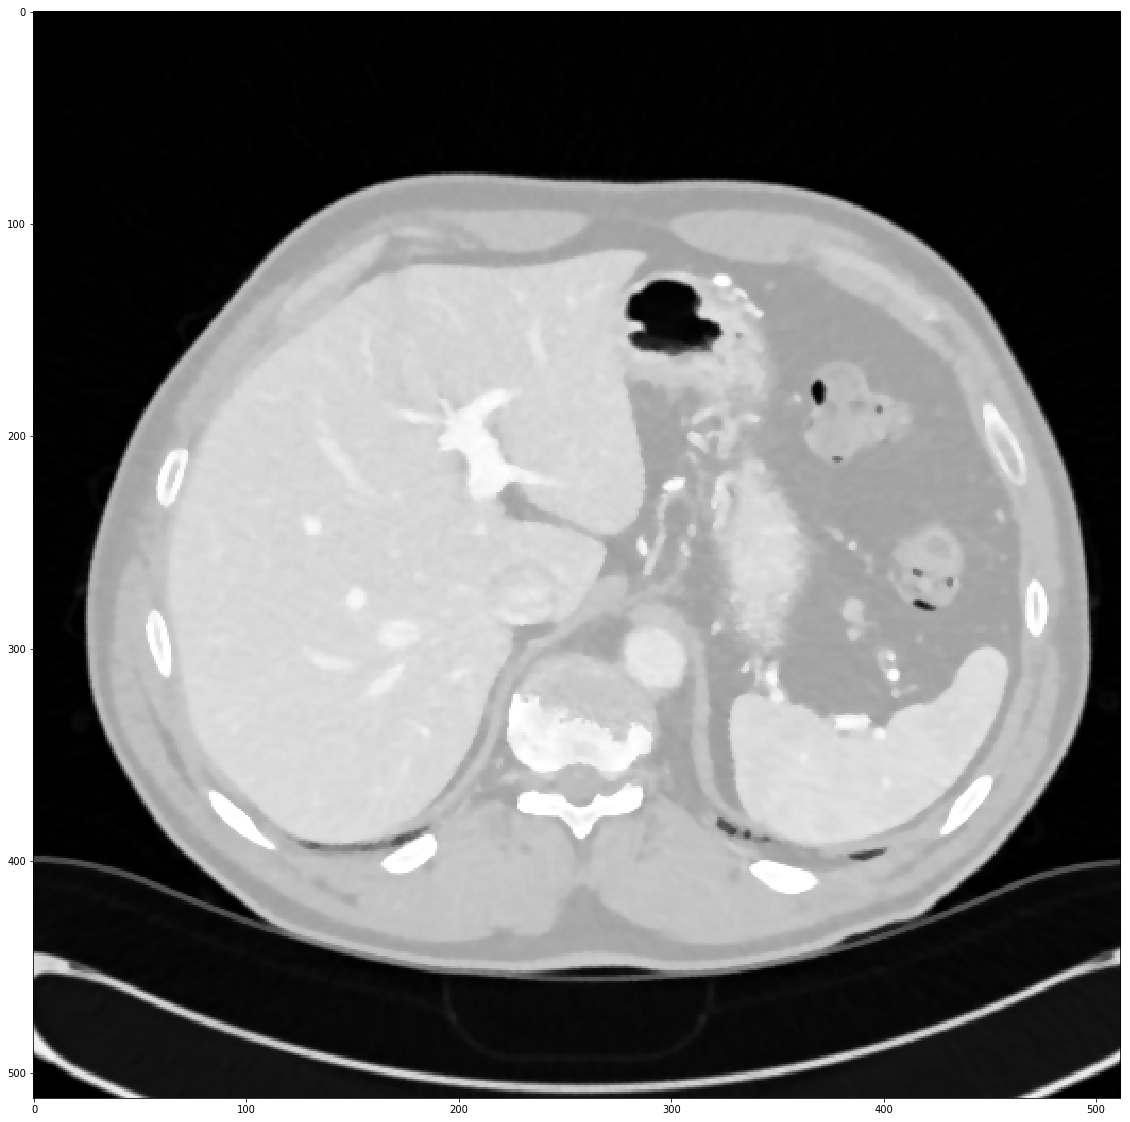
\includegraphics[width=0.3\textwidth]{Images/Liver_rm_noise.png}%
    \label{fig:c}%
    }% 
  \caption{Minh hoạ quá trình tiền xử lý một lát cắt trên ảnh CT}
  \label{fig:ab}
\end{figure*}

\subsection{Loại bỏ nhiễu}
Chúng tôi đã sử dụng công cụ Isotropic diffusion filter trong thư viện SimpleItk để loại bỏ nhiểu. Các tham số sử dụng:
\begin{itemize}
    \item Iterations: 10
    \item TimeStep: 0.625
    \item Conductance Parameter: 1.5
\end{itemize}
\subsection{Isometric}
Dữ liệu trên các tập SLIVER07, 3Dircadb và LITS2017 có khoảng cách giữa các voxel (spacing) rất khác nhau sẽ gây khó khăn cho mô hình phân đoạn. Đặc biệt là khoảng cách giữa các voxels trục Z ứng với khoảng cách giữa các lát cắt nằm trong khoảng rất lớn, từ 0.5 mm đến 6 mm. Vì vậy, chúng tôi đã đồng bộ khoảng cách giữa các voxels trên tất cả các trục về 1 (mm) đối với tất cả các mẫu dữ liệu. Việc này được thực hiện bằng công cụ Zoom trong thư viện Scipy với nội suy Cubic Spline, $Zoom = (Spacing_x, Spacing_y, Spacing_z)$.


\chapter{Huấn luyện, cải tiến và kiểm thử mô hình}
\section{Mô hình 2D}
\section{Mô hình 3D}



\chapter{Hậu xử lý kết quả}
\section{Loại bỏ khối}
\section{Lấp đầy khối}
\section{Làm mượt bằng màng lọc}
\section{Làm mượt bằng trường điều kiện ngẫu nhiên}






\chapter{Tổng hợp, so sánh kết quả hệ thống phân đoạn với những phương pháp khác}
Để có một nhận định, đánh giá khách quan với hệ thống phân đoạn, chúng tôi đã thực hiện đánh giá trên những tập dữ liệu khác nhau SLIVER07, 3Dircadb,  LiTS2017. Từ đó, chúng tôi đã tổng hợp kết quả, so sánh với những hệ thống phân đoạn khác trên cùng tập dữ liệu kiểm thử.
\section{3D Image Reconstruction for Comparison of Algorithm Database (3Dircadb)}
Trong phần này, chúng tôi so sánh kết quả dự đoán của hai mô hình: mạng nơ-ron tích chập 3-chiều (CNN 3D) và TLUnet3D với 20 ảnh chụp cắt lớp vi tính trong tập 3Dircadb\_1. Các kết quả chúng tôi sử dụng để so sánh bao gồm các phương pháp: Duy \cite{Duy_paper}, Chartrand và cộng sự \cite{Chartrand_paper}, Patrick và cộng sự \cite{Patrick_paper}, Qiangguo và cộng sự  \cite{Qiangguo_paper}, Xiaomeng và cộng sự  \cite{Xiaomeng_paper}. Trong đó, phương pháp Chartrand \cite{Chartrand_paper} là phương pháp bán tự động. Các phương pháp còn lại đều là phương pháp tự động. Phương pháp của Duy \cite{Duy_paper} và phương pháp của Patrick và cộng sự\cite{Patrick_paper} đều sử dụng mạng học sâu Unet 2-chiều và sử dụng trường điều kiện ngẫu nhiên (3D Dense CRFs) để thực hiện hậu xử lý. Phương pháp Qiangguo\cite{Qiangguo_paper} và phương pháp Xiaomeng \cite{Xiaomeng_paper} đều sử dụng mạng học sâu Unet 3-chiều với một số biến đổi (RA-UNet và H-DenseUNet) và cả hai phương pháp này đều đạt kết quả rất tốt. Mô hình TLUnet3D (đề xuất) cũng đã đạt được kết quả rất tốt trên tập 3Dircadb. Một số kết quả dự đoán bằng mô hình TLUnet3D đã đạt với 99\%  Dice per case.
\begin{table}[]
\begin{adjustwidth}{-1.8cm}{}
\begin{tabular}{lcccccc}
\hlineB{6}
\textbf{Phương pháp} & \textbf{Dice per case} & \textbf{VOE}         & \textbf{RVD}          & \textbf{AvgD}        & \textbf{RMSD}        & \textbf{MaxD}        \\ \hlineB{6}
Duy \cite{Duy_paper}                 & 94.58 ± \_             & 10.28 ± \_           & \_                    & \_                   & \_                   & \_                   \\ \hline
Chartrand et al. \cite{Chartrand_paper}            & 97.17 ± \_             & 5.50 ± 1.00          & -0.10 ± 2.40          & 2.00 ± 0.30          & \_                   & \_                   \\ \hline
Patrick et al. \cite{Patrick_paper}              & 94.3 ± \_              & 10.07 ± \_           & -1.4 ± \_             & 1.5 ± \_             & \_                   & 24 ± \_              \\ \hline
Qiangguo et al. \cite{Qiangguo_paper}        & 	97.7 ± \_           & 4.50 ± \_          & -0.1 ± \_         & 0.587 ± \_            & \_          & 18.617 ± \_         \\ \hline
Xiaomeng et al. \cite{Xiaomeng_paper}        & 	98.2 ± 1.00           & 3.57 ± 1.66          & \textbf{0.01 ± 0.02}         & 1.28 ± 2.02         & 3.58 ± 6.58          &  \_         \\ \hlineB{4}
CNN 3D        & 97.60 ± 0.41           & 4.69 ± 0.79          & -0.24 ± 1.26          & 0.59 ± 0.12          & 1.21 ± 0.35          & 17.42 ± 7.13         \\ \hline
TLUnet3D         & \textbf{98.69 ± 0.53}  & \textbf{2.58 ± 1.02} & -0.14 ± 0.77 & \textbf{0.26 ± 0.17} & \textbf{0.55 ± 0.30} & \textbf{7.83 ± 7.14} \\ \hlineB{6}
\end{tabular}
\caption{\label{tab:compare_3Dircadb}So sánh kết quả 20 bệnh nhân tập dữ liệu 3Dircadb\_1}
\end{adjustwidth}
\end{table}
\section{Segmentation of the Liver 2007 (SLIVER07)}
Chúng tôi đã thực hiện phân đoạn lá gan trên tập kiểm thử của cuộc thi này và gởi kết quả dự đoán đến ban tổ chức cuộc thi để nhận được đánh giá. Tuy nhiên, cuộc thi này đã ngừng hệ thống đánh giá trước khi chúng tôi hoàn thành mô hình TLUnet3D. Vì vậy, chúng tôi chỉ nhận được kết quả đánh giá phân đoạn trên hai mô hình 2-chiều và mô hình nơ-ron tích chập 3-chiều (CNN 3D). Bảng \ref{tab:compare_SLIVER07} cho thấy so sánh đánh giá kết quả dự đoán với những phương pháp tốt nhất, bao gồm: Maklad và cộng sự \cite{Maklad_paper}, Beichel và cộng sự \cite{Beichel_paper}, Afifi và Nakaguchi \cite{Afifi_paper}, Peng và cộng sự \cite{Peng_paper} \cite{Peng_Wang_paper} \cite{Peng_Dong_paper}, Kainmuller và cộng sự \cite{Kainmuller_paper}, Wimmer và cộng sự \cite{Wimmer_paper}, Qi Dou và cộng sự \cite{dsn_paper}. Ngoài "Final Score", chi tiết về trung bình của tất cả năm độ đo cũng được liệt kê. Phương pháp của Beichel \cite{Beichel_paper} là phương pháp thủ công (tương tác), đòi hỏi trung bình 16 phút cho mỗi mẫu dữ liệu. Năm phương pháp bao gồm Maklad \cite{Maklad_paper}, Afifi \cite{Afifi_paper}, Peng \cite{Peng_Wang_paper}, Peng \cite{Peng_Dong_paper}, Wimmer \cite{Wimmer_paper} đều là phương pháp bán tự động với những yêu cầu khác nhau trong tương tác. Những tương tác này bao gồm rất nhiều bước để xác định được những đặc trưng như lá lách, mạch máu, phân loại mạch máu gan hoặc mạch máu không phải của gan. Ngoài ra, phương pháp  Peng \cite{Peng_paper}, Kainmuller \cite{Kainmuller_paper}, Qi Dou \cite{dsn_paper}, và các phương pháp của chúng tôi đều là phương pháp tự động. Phương pháp Peng \cite{Peng_paper} sử dụng kỹ thuật Graph-Cut. Phương pháp Kainmuller \cite{Kainmuller_paper} dựa trên kỹ thuật "Support Vector Machine". Và phương pháp Qi Dou \cite{dsn_paper} chính là phương pháp chúng tôi đã tham khảo cho mô hình CNN 3D. Ngoài kỹ thuật sử dụng mạng nơ-ron học sâu thì phương pháp này còn sử dụng trường điều kiện ngẫu nhiên (3D Dense CRFs) để thực hiện hậu xử lý. Kỹ thuật CRFs này đòi hỏi rất nhiều bộ nhớ cũng như thời gian tính toán để thực hiện.
\begin{table}[]
\begin{adjustwidth}{-1.8cm}{}
\begin{tabular}{lcccccc}
\hlineB{6}
\textbf{Phương pháp}                            & \textbf{Score} & \textbf{VOE} & \textbf{RVD} & \textbf{AvgD} & \textbf{RMSD} & \textbf{MaxD} \\ \hlineB{6}
Maklad et al \cite{Maklad_paper}                                          & \textbf{85.7 ± 2.5}     & \textbf{4.33 ± 0.69}  & \textbf{0.28 ± 0.82}  & \textbf{0.63 ± 0.15}   & \textbf{1.19 ± 0.26}   & \textbf{14.01 ± 2.73}  \\ \hline
Beichel et al. \cite{Beichel_paper}                                         & 82.1 ± 2.8     & 5.18 ± 0.89  & 0.96 ± 1.62  & 0.79 ± 0.18   & 1.43 ± 0.36   & 15.69 ± 3.30  \\ \hline
Afifi et al. \cite{Afifi_paper}                                           & 81.7 ± 3.8     & 5.03 ± 0.87  & 1.83 ± 1.24  & 0.74 ± 0.16   & 1.52 ± 0.38   & 16.59 ± 3.89  \\ \hline
Peng et al. \cite{Peng_paper}                                            & 83.4 ± 3.1     & 4.58 ± 0.51  & 1.08 ± 0.80  & 0.68 ± 0.14   & 1.45 ± 0.36   & 16.88 ± 3.68  \\ \hline
Peng et al. \cite{Peng_Wang_paper}                                            & 80.6 ± 3.5     & 5.45 ± 0.82  & 1.03 ± 1.61  & 0.82 ± 0.14   & 1.68 ± 0.40   & 18.59 ± 4.31  \\ \hline
Peng et al. \cite{Peng_Dong_paper}                                            & 80.0 ± 4.0     & 6.07 ± 1.13  & -0.04 ± 2.15 & 0.92 ± 0.23   & 1.61 ± 0.44   & 16.82 ± 2.32  \\ \hline
Kainmuller et al. \cite{Kainmuller_paper}                                      & 77.3 ± 8.9     & 6.09 ± 2.02  & -2.86 ± 2.76 & 0.95 ± 0.33   & 1.87 ± 0.76   & 18.69 ± 8.02  \\ \hline
Wimmer et al. \cite{Wimmer_paper}                                          & 76.8 ± 3.8     & 6.47 ± 0.92  & 1.04 ± 2.67  & 1.02 ± 0.16   & 2.0 ± 0.35    & 18.32 ± 4.66  \\ \hline
Qi Dou et al. \cite{dsn_paper}                                          & \_             & 5.42 ± 0.72  & 1.75 ± 1.77  & 0.79 ± 0.14   & 1.64 ± 0.34   & 33.55 ± 19.64 \\ \hlineB{4}
Model 2D  & 71.51 ± 11.25  & 6.63 ± 2.02  & -0.31 ± 4.02        & 1.15 ± 0.45   & 2.64 ± 1.36   & 26.49 ± 13.47 \\ \hline
CNN 3D  & 79.89 ± 4.57   & 5.58 ± 0.90  & -0.19 ± 1.34 & 0.86 ± 0.14   & 1.77 ± 0.53   & 20.79 ±  7.94 \\ \hlineB{6}
\end{tabular}
\caption{\label{tab:compare_SLIVER07}So sánh kết quả 10 bệnh nhân trên tập dữ liệu kiểm thử SLIVER07}
\end{adjustwidth}
\end{table}
\section{Liver Tumor Segmentation Challenge (LITS2017)}
Hiện nay, Liver Tumor Segmentation Challenge Open Leaderboard \cite{website:LiTS_learderboard}  đã đánh giá được rất nhiều kết quả phân đoạn gan và khối u. Tuy nhiên, chúng tôi chỉ liệt kê những kết quả của những phương pháp có bài báo công khai, bao gồm: Bi và cộng sự  \cite{Lei_paper}, Kaluva và cộng sự  \cite{Krishna_paper}, Qiangguo và cộng sự  \cite{Qiangguo_paper}, Xiaomeng và cộng sự  \cite{Xiaomeng_paper} . Ngoài ra, chúng tôi sẽ so sánh với phương pháp Nhật và Sơn \cite{Beichel_paper}. Tất cả những phương pháp phân đoạn lá gan chúng tôi đã liệt kê trong phần này đều là phương pháp tự động hoàn toàn và  sử dụng mô hình mạng học sâu. Kaluva và cộng sự  \cite{Krishna_paper} đã sử dụng mạng Unet 2-chiều và đạt 92.30 \% Dice global. Phương pháp của Kaluva và cộng sự  \cite{Krishna_paper}, phương pháp Nhật và Sơn \cite{Beichel_paper} dùng mạng học sâu với kiến trúc Resnet 2-chiều đã đạt kết quả khả quan hơn với 96.50 \% Dice global. Những phương pháp còn lại, Qiangguo và cộng sự  \cite{Qiangguo_paper}, Xiaomeng và cộng sự  \cite{Xiaomeng_paper} đều là phương pháp sử dụng kiến trúc giống với Unet 3-chiều và đạt được kết quả rất tốt với 96.50\% và 96.30\% Dice global. Mô hình TLUnet3D của chúng tôi cũng đã đạt kết quả dự đoán rất tốt trong thử thách này với 96.60\% Dice global và nằm trong Top 5 Dice Global, Top 7 Dice per case trên LITS2017 Open Leaderboard \cite{website:LiTS_learderboard}.

\begin{table}[]
\begin{adjustwidth}{-0.2cm}{}
\begin{tabular}{lccccccc}
\hlineB{6}
\textbf{Phương pháp} & \textbf{Dice global} & \textbf{Dice per case} & \textbf{VOE} & \textbf{RVD} & \textbf{AvgD} & \textbf{RMSD} & \textbf{MaxD} \\ \hlineB{6}
Bi et al. \cite{Lei_paper}            & \_                   & 95.90                  & 7.80         & \_           & \_            & \_            & \_            \\ \hline
Kaluva et al. \cite{Krishna_paper}        & 92.30                & 91.20                  & 15.00        & -0.80         & 6.47          & \_            & 45.93         \\ \hline
Qiangguo et al. \cite{Qiangguo_paper}      & 96.30                & 96.10                  & 7.40         & 0.20          & 1.21         & 2.81          & 26.95        \\ \hline
Xiaomeng et al.  \cite{Xiaomeng_paper}      & 96.50                & 96.10                  & 7.40        & -1.80       & 1.45         & \_            & 27.12        \\ \hline
Nhat et al. \cite{Beichel_paper}          & 96.50                & 96.10                  & 7.40         & -2.30        & \_            & \_            & \_            \\ \hlineB{4}
CNN 3D     & 95.80                & 95.30                  & 8.80         & 2.60         & 1.44          & 2.82          & 24.94         \\ \hline
TLUnet3D   & 96.60                & 96.00                  & 7.60         & 2.00          & 1.20          & 2.54          & 23.92         \\ \hlineB{6}
\end{tabular}
\caption{\label{tab:compare_SLIVER07}So sánh kết quả 70 bệnh nhân trên tập dữ liệu kiểm thử LITS2017}
\end{adjustwidth}
\end{table}
\section{Mô hình đề xuất}
Trên đây là kết quả so sánh giữa các mô hình của chúng tôi với các mô hình khác đã được công bố công khai. Qua các kết quả này, chúng tôi đề xuất mô hình TLUnet3D là mô hình tốt nhất mà qua luận văn này chúng tôi nghiên cứu được.



\chapter{Xây dựng ứng dụng}
Để hiển thị kết quả của mô hình một cách trực quan thì nhóm đã xây dựng một ứng dụng hiển thị trên website cho phép người dùng upload dữ liệu, sau đó hiển thị kết quả phân đoạn và mô hình 3D. Phần này sẽ trình bày về cấu trúc, luồng xử lý, cách xây dựng và các chức năng chính của ứng dụng.
\section{Cấu trúc ứng dụng}
Ứng dụng được xây dựng theo mô hình client - server API (gồm hai phần là client và server riêng biệt hoạt động với nhau qua cơ chế gọi API).
\begin{figure}[h]
\centering
    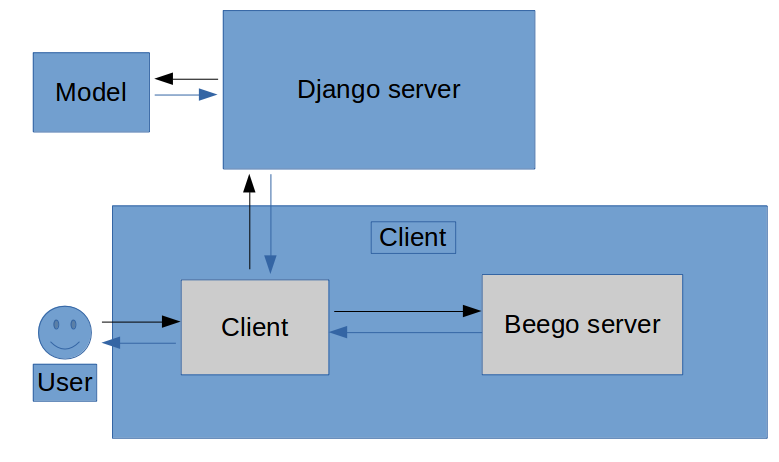
\includegraphics[totalheight=7cm]{Images/app_struct.png}
    \caption{Cấu trúc chính của ứng dụng}
    \label{skip_conn}
\end{figure}
\section{RESTful API}
REST (Representational State Transfer) ra đời vào năm 2000 bởi Roy Thomas Fielding. Ta có thể gọi đây là các ràng buộc và quy ước mà khi hệ thống nào làm theo thì được gọi là REST.\\
API (Application Programming Interface) là phương thức để kết nối các thư viện và ứng dụng với nhau \cite{website:api}.\\

RESTful API là một tiêu chuẩn dùng trong việc thết kế các thiết kế API cho các ứng dụng web để quản lý các tài nguyên. RESTful là một trong những kiểu thiết kế API được sử dụng phổ biến nhất ngày nay \cite{website:restfulapi}.\\
Về cơ bản thì RESTful API là một khái niệm khá trừu tượng nhưng lại rất dễ sử dụng. Để cho dễ hiểu thì phần này sẽ trình bày về cấu trúc và cách sử dụng, đồng thời gọi tắt là ``API`` cho cơ chế này.\\
Cấu trúc của một RESTful API gồm những phần như sau:
\begin{itemize}
    \item METHOD (bắt buộc): Gồm các phương thức cơ bản như GET, POST, PUT, DELETE.
    \item URL (bắt buộc): đường dẫn của API(đường dẫn này sẽ được phân chia trong Routers bên phía server).
    \item DATA (tùy chọn): đối tượng JSON mô tả dữ liệu kèm theo gửi lên server.
    \item HEADER (tùy chọn): Đối tượng JSON thường dùng trong việc bảo mật và xác thực người dùng.
    \item PARAM (tùy chọn): Các tham số đi kèm sau dấu ``?`` của URL.
\end{itemize}
Các bước gọi và phản hồi API cơ bản như sau:
Phía client tạo một API chứa những thông tin cần thiết như trên, phía server sẽ kiểm tra header có phù hợp hay không, sau đó nhận dữ liệu, kiểm tra tính hợp lệ của dữ liệu, xử lý và trả lại dữ liệu cần thiết cho client nếu có.
\begin{figure}[h]
\centering
    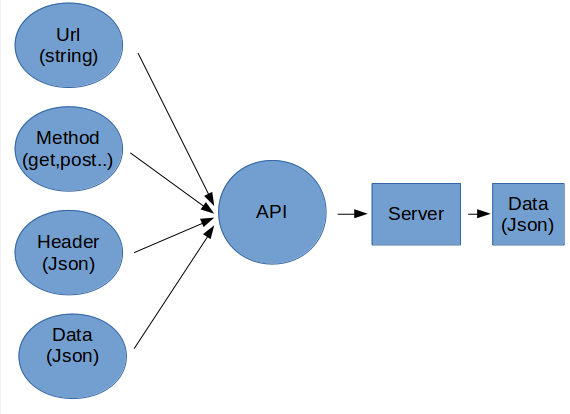
\includegraphics[totalheight=7cm]{Images/app_json.png}
    \caption{Cấu trúc và luồng xử lý của một API}
    \label{skip_conn}
\end{figure}
\section{Các ngôn ngữ, framework và các thư viện liên quan}
Phần này sẽ trình bày sơ qua về các ngôn ngữ lập trình, các framework và các thư viện liên quan được sử dụng để xây dựng ứng dụng.
\subsection{Ngôn ngữ Python}
Python là một ngôn ngữ bậc cao, mã nguồn mở ra mắt lần đầu vào năm 1991 bởi Guido van Rossum. Hiện tại thì nó có hai phiên bản phổ biến là Python 2 và Python 3(trong ứng dụng sử dụng Python 3 bản 3.5.2).\\
Một số ưu điểm của Python như sau:
\begin{itemize}
    \item Cú pháp đơn giản, cấu trúc rõ ràng, dễ đọc dễ học nên code ngắn gọn nhưng đem lại hiệu quả cao.
    \item Có rất nhiều thư viện và framework hỗ trợ đặc biệt trong việc xây dựng các ứng dụng về học máy, đồng thời cộng đồng hỗ trợ rất nhiều nên dễ dàng được hỗ trợ khi gặp khó khăn.
    \item Dễ dàng kết hợp với các ngôn ngữ khác.
\end{itemize}
Với những ưu điểm nêu trên, Python được sử dụng khá rộng rãi trong việc lập trình game, website và đặc biệt là lập trình các hệ thống học máy đang hot hiện nay.\\

Để biết thêm về Python có thể tham khảo tại \href{https://docs.python.org}{đây}.
\subsection{Framework Django}
Django là framework phổ biến nhất của Python và được viết hoàn toàn bằng Python, ra đời vào năm 2005 bởi Adrian Holovaty và Simon Willison. Django chủ yếu được sử dụng để xây dựng các ứng dụng website theo mô hình Model-View-Template (MVT) với ngôn ngữ xử lý phía server là Python. Django server cung cấp cơ chế phục vụ API cho các client gọi vào. Phần ứng dụng của nhóm chỉ sử dụng tới cơ chế này nên sẽ không trình bày nhiều về framework Django. Để biết thêm về framework Django có thể tham khảo tại \href{https://docs.djangoproject.com/en/2.2/}{đây}. 
\subsection{Các thư viện hỗ trợ trong Python}
Để cho việc lập trình được nhanh chóng thì ứng dụng sử dụng rất nhiều các thư viện của Python, đặc biệt có thể kế đến như:
\begin{itemize}
    \item zipfile: hỗ trợ việc nén/giải nén file.
    \item SimpleITK: hỗ trợ việc đọc file dạng raw/mhd nhanh chóng.
    \item numpy: hỗ trợ việc tính toán nhanh chóng, đặc biệt trên các mảng nhiều chiều.
    \item csv: hỗ trợ đọc và ghi file csv.
    \item skimage: cung cấp module measure để tạo tập đỉnh và mặt từ mảng ba chiều.
\end{itemize}
\subsection{Ngôn ngữ Golang}
Golang hay còn được gọi là Go được thiết kế và phát triển bởi Robert Griesemer, Rob Pike và Ken Thompson tại Google vào năm 2007, được giới thiệu vào năm 2009 và hiện tại được sử dụng trong hầu hết trong các sản phẩm của Google. Hiện tại thì Go khá được ưa chuộng bởi các đặc điểm sau \cite{website:golang}:
\begin{itemize}
    \item Hỗ trợ khai báo kiểu dữ liệu động.
    \item Tốc độ biên dịch nhanh.
    \item Hỗ trợ các tác vụ đồng thời.
    \item Ngôn ngữ đơn giản, ngắn gọn.
\end{itemize}
Nói tóm lại, Go có tốc độ xử lý nhanh tương đương như C/C++ nhưng cấu trúc đơn giản và hỗ trợ trình dọn rác tự động nên dễ sử dụng, hiệu quả cao. Để biết thêm thông tin về Go thì có thể tham khảo tại \href{https://golang.org/doc/}{đây}. 
\subsection{Framework Beego}
Beego là một framework mã nguồn mở cho cộng đồng sử dụng miễn phí và phát triển nó theo đường dẫn \href{https://github.com/astaxie/beego}{này}.\\
Ta sử dụng Beego để tạo một ứng dụng web chạy trực tiếp trên máy chủ local. Khi cài đặt và tạo một dự án bằng Beego, ta sẽ có một cây thư mục hoàn chỉnh cho các thành phần chính của ứng dụng.\\
\begin{figure}[h]
\centering
    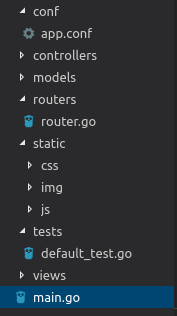
\includegraphics[totalheight=7cm]{Images/app_beego_struct_folder.png}
    \caption{Cây thư mục làm việc trong Beego}
    \label{skip_conn}
\end{figure}
Ứng dụng web được tạo bởi Beego theo mô hình Model-View-Controller (MVC) và giao tiếp qua cơ chế gọi API, các thành phần của ứng dụng được giải thích ngắn gọn như sau:
\begin{itemize}
    \item Conf: chứa file config định nghĩa một số thông tin chính như cổng, tên, thông tin cơ sở dữ liệu…
    \item Controllers: Nhận và xử lý dữ liệu từ bên ngoài, rồi gọi tới Model và gửi dữ liệu ra nếu có.
    \item Main.go: File để chạy ứng dụng.
    \item Models: Nhận dữ liệu đã hợp lệ từ Controllers để xử lý, thường là các tác vụ liên quan tới cơ sở dữ liệu và trả về dữ liệu cần thiết cho Controller.
    \item Routers: Quản lý, phân chia các API cho các Controller tương ứng.
    \item Static: chứa các dữ liệu cần thiết cho phía client.
    \item Tests: Dùng để kiểm tra lại ứng dụng, là nơi làm việc của kiểm tra viên.
    \item Views: Mặc định chứa file hiển thị trang chủ.
\end{itemize}
Để tìm hiểu kĩ hơn về framework Beego có thể tham khảo tại \href{ https://beego.me/docs}{đây}.

\subsection{Framework AngularJS}
AngularJS có thể gọi là một framework được viết bằng Javascript. AngularJS đưa ra hướng dẫn cụ thể trên mã lệnh HTML với các tiền tố ``ng-`` hay còn được gọi là directives \cite{website:angularjs}.\\
Để sử dụng thì chỉ cần nhúng đường dẫn tới file angular.min.js như sử dụng các thư viện của Javascript.\\
Một số directive quan trọng có thể kể đến như sau:
\begin{itemize}
    \item ng-app: Đánh dấu thẻ HTML mà AngularJS được bắt đầu sử dụng.
    \item ng-model: giá trị HTML trong thẻ này tương đương với biến \$scope trong phần Controller tương ứng.
    \item ng-change, ng-click: bắt sự kiện thay đổi, click để gọi hàm \$scope tương ứng.
\end{itemize}
Một điều quan trọng nữa là AngularJS hỗ trợ gọi API để gửi và nhận dữ liệu một cách dễ dàng qua biến \$http.
Để biết thêm về AngularJS có thể tham khảo tại \href{ https://docs.angularjs.org/api/ng/service/\$document
}{đây}.
\subsection{Một số thư viện khác hỗ trợ phần hiển thị}
Ngoài những thư viện và framework quan trọng kể trên thì ứng dụng của nhóm sử dụng khá nhiều các thư viện hỗ trợ phần thiết kế giao diện như:
\begin{itemize}
    \item Bootstrap: Thư viện quen thuộc để xây dựng giao diện responsive dễ dàng. Trong ứng dụng này sử dụng bootstrap phiên bản 3.3.7.
    \item Plotly: Thư viện giúp hiển thị hình ảnh 3D từ file csv chứa tập đỉnh và mặt.
    \item Jquery, Font Awesome, Rangesslider: hỗ trợ việc hiển thị được tốt và hiệu quả hơn.
\end{itemize}
\section{Xây dựng phần Django server}
Phần server chính của ứng dụng (Django server) được xây dựng bằng ngôn ngữ Python với framework là Django, làm việc trực tiếp với mô hình đã huấn luyện được và server này sẽ cung cấp một API để client gọi vào. 
\begin{figure}[h]
\centering
    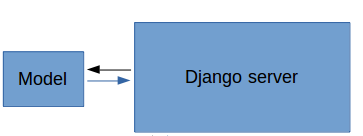
\includegraphics[totalheight=5cm]{Images/app_posdjangoserver.png}
    \caption{Vị trí Django server trong cấu trúc ứng dụng}
    \label{skip_conn}
\end{figure}
Luồng xử lý phần server này được chia làm các giai đoạn như sau: 
\begin{itemize}
    \item Quá trình xử lý dữ liệu đầu vào và chạy model.
    \item Quá trình xử lý sau chạy model.
    \item Tạo đối tượng JSON và gửi cho client.
\end{itemize}
\begin{figure}[h]
\centering
    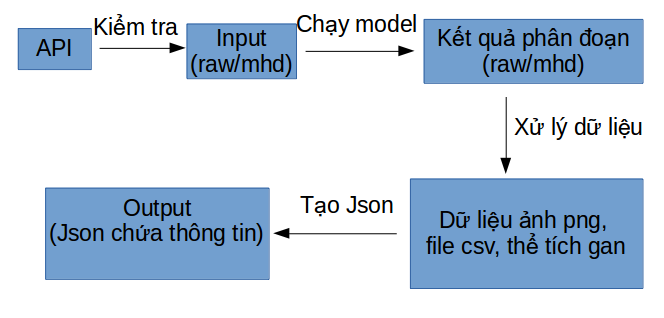
\includegraphics[totalheight=7cm]{Images/app_django_struct.png}
    \caption{Luồng xử lý trong Django server}
    \label{skip_conn}
\end{figure}
\subsection{Quá trình xử lý dữ liệu đầu vào và chạy model}
Dữ liệu đầu vào để server xử lý phải là dữ liệu có định dạng raw/mhd (định dạng như tập Sliver07). Dữ liệu có thể chỉ cần tập ảnh scan nếu muốn phân đoạn hoặc bao gồm cả tập nhãn nếu muốn so sánh và đánh giá kết quả phân đoạn.\\
Sau khi nhận dữ liệu đầu vào dưới dạng API, server sẽ tiến hành kiểm tra API này, sau đó lấy dữ liệu và lưu lại, chạy model để cho ra kết quả phân đoạn. Đầu ra của quá trình này cũng là file có định dạng raw/mhd. Thời gian chạy cho quá trình này mất khá nhiều thời gian khi chạy trên máy local không có GPU.
\begin{figure}[h]
\centering
    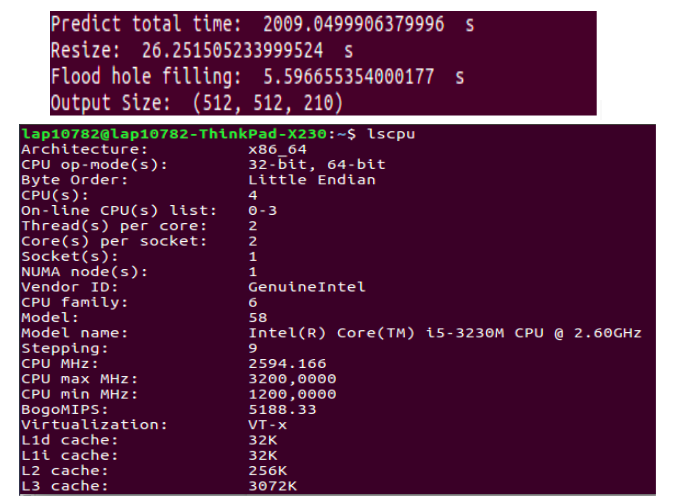
\includegraphics[totalheight=7cm]{Images/app_configuration.png}
    \caption{Thời gian chạy model với cấu hình máy tương ứng}
    \label{skip_conn}
\end{figure}
\subsection{Quá trình xử lý sau chạy model}
Khi chạy xong model, sử dụng các thư viện hỗ trợ của Python để xử lý dữ liệu như sau:
\begin{itemize}
    \item Thư viện SimpleITK đọc hình ảnh dạng raw/mhd ra các thông tin cần thiết như mảng chứa nội dung các hình ảnh, spacing của dữ liệu, từ đó tính thể tích một cách dễ dàng.
    \item Thư viện numpy xử lý các mảng dữ liệu để ra các hình ảnh dạng so sánh, dán kết quả lên scan.
    \item Module measure trong thư viện skimage tạo tập đỉnh và mặt từ mảng hình ảnh phân đoạn, sau đó dùng thư viện csv để đọc và ghi các tập đỉnh và mặt này vào file.
\end{itemize}
Tất các các hình ảnh đầu ra của quá trình này đều có định dạng là png. Sau khi tạo các thông tin đó thì tạo file zip kèm theo cho mỗi tập. Các tập dữ liệu tạo ra tương ứng như sau:
\begin{itemize}
    \item Với tập đầu vào chỉ có scan, kết quả của quá trình này sẽ bao gồm: Tập ảnh scan, tập ảnh kết quả phân đoạn, tập ảnh phân đoạn dán lên scan, file csv gồm thông tin tập đỉnh và mặt của mô hình gan 3D, thể tích gan theo kết quả phân đoạn.
    \item Với tập có cả scan và nhãn thì kết quả bao gồm: Tập ảnh scan, tập ảnh nhãn, tập ảnh kết quả phân đoạn so sánh với nhãn,  tập ảnh kết quả phân đoạn so sánh với nhãn dán lên scan, file csv gồm thông tin tập đỉnh và mặt mô hình gan 3D và thể tích gan của kết quả phân đoạn và của nhãn.
\end{itemize}


\begin{figure}[h]
\centering
    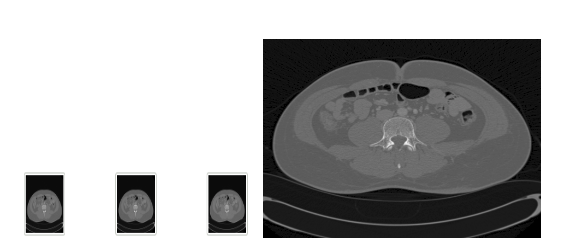
\includegraphics[totalheight=7cm]{Images/app_listscan.png}
    \caption{Tập ảnh scan được lưu lại}
    \label{skip_conn}
\end{figure}


\begin{figure}[h]
\centering
    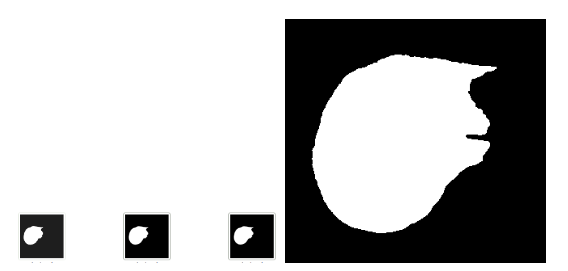
\includegraphics[totalheight=7cm]{Images/app_listlabel.png}
    \caption{Tập ảnh phân đoạn/nhãn được lưu lại}
    \label{skip_conn}
\end{figure}

\begin{figure}[h]
\centering
    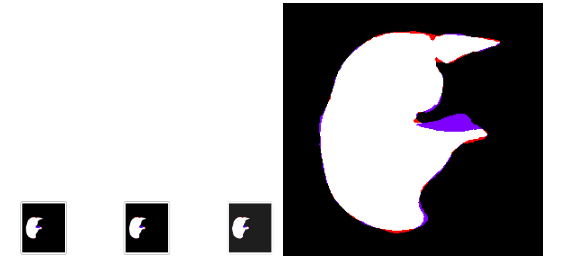
\includegraphics[totalheight=7cm]{Images/app_listcompare.png}
    \caption{Tập ảnh phân đoạn so sánh với nhãn được lưu lại(nếu có nhãn)}
    \label{skip_conn}
\end{figure}


\begin{figure}[h]
\centering
    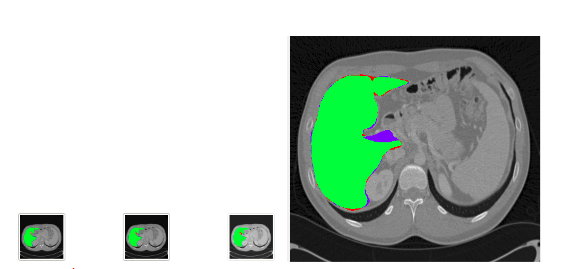
\includegraphics[totalheight=7cm]{Images/app_listoverlap.png}
    \caption{Tập ảnh kết quả dán lên scan}
    \label{skip_conn}
\end{figure}

\subsection{Tạo đối tượng JSON và gửi cho client}
Với cơ chế gọi API, dữ liệu nhận và gửi sẽ ở định dạng JSON nên dữ liệu trả về cho client sẽ là một đối tượng JSON với các trường dữ liệu được mô tả như sau (các đường dẫn tương ứng là các file đã được lưu trong server):
\begin{itemize}
    \item ListPredict: mảng các đường dẫn của ảnh kết quả phân đoạn.
    \item ListLabel: mảng các đường dẫn của ảnh nhãn(nếu có).
    \item ListOverlap: mảng các đường dẫn ảnh kết quả dán lên scan.
    \item CsvFileLabel: đường dẫn tới file csv của nhãn(nếu có).
    \item CsvFilePredict: đường dẫn tới file csv kết quả phân đoạn.
    \item LinkZip: đối tượng json chứa các đường dẫn tới file zip của các tập.
    \item VolumePredict: thông tin thể tích theo kết quả phân đoạn.
    \item VolumePredict: thông tin thể tích theo kết quả phân đoạn.
\end{itemize}
Sau khi tạo xong đối tượng json sẽ được gửi về client xử lý.

\section{Xây dựng phần client}
Với cấu trúc server như trên chúng ta có thể xây dựng phần client một cách linh động sao cho trực quan nhất trên bất cứ nền tảng nào qua cơ chế API. Ở phần này thì nhóm xây dựng phần client này trên nền tảng website sử dụng framework Beego, với ngôn ngữ phía server là Golang, phía client là HTML, CSS, Javascript cho giao diện, sử dụng framework AngularJS để giao tiếp với phía server Golang.
\begin{figure}[h]
\centering
    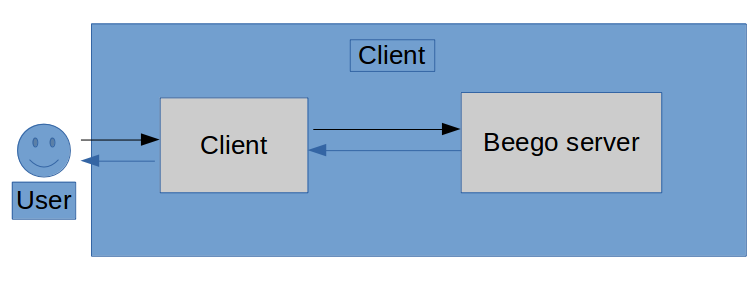
\includegraphics[totalheight=5cm]{Images/app_postclient.png}
    \caption{Vị trí phần client trong cấu trúc ứng dụng}
    \label{skip_conn}
\end{figure}
Các công việc chính theo thứ tự của phần client này như sau:
\begin{itemize}
    \item Upload dữ liệu và lấy đường dẫn cần thiết từ Django server.
    \item Beego server thực hiện việc tải về, giải nén các file từ đường dẫn.
    \item Beego server tạo đối tượng JSON để gửi lại cho giao diện hiển thị.
\end{itemize}

\begin{figure}[h]
\centering
    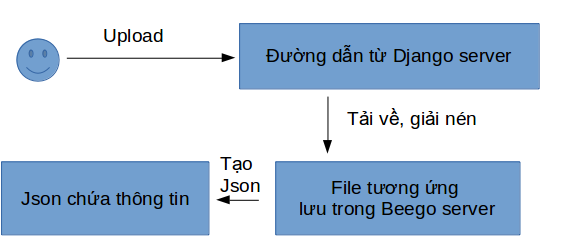
\includegraphics[totalheight=7cm]{Images/app_beego_struct.png}
    \caption{Luồng xử lý phần client chính}
    \label{skip_conn}
\end{figure}

\paragraph{Upload dữ liệu:} Khi upload dữ liệu dạng file zip, phía client Javascript phải tạo dữ liệu để gọi API lên Django server. Dữ liệu này là một đối tượng JSON không giống thông thường mà nó phải khai báo kiểu FormData() mới lưu trữ được nội dung file mà người dùng upload qua thẻ input.\\
\paragraph{Công việc của Beego server:} Ngoài việc tạo đường dẫn trên máy chủ, Beego sẽ nhận các đường dẫn các file trong Django server từ client qua API, sau đó thực hiện việc giải nén và tạo file lưu trữ nội dung của lần phân đoạn sau cùng. Sau đó tạo đối tượng JSON để gửi lại dữ liệu cho client qua việc phản hồi API.
\paragraph{Hiển thị mô hình 3D:} Như đã nêu ở trên, việc hiển thị mô hình 3D của lá gan sẽ dùng tới thư viện Plotly. Chỉ cần nhúng file plotly.js vào, ta có thể đọc file csv chứa tập đỉnh và mặt do Django server đã tạo, sau đó tạo một đối tượng JSON chứa các tập đỉnh và mặt này và tiếp tục dùng Plotly để đọc đối tượng JSON và tạo ra mô hình 3D với kiểu hiển thị là "mesh3D".

\begin{figure}[h]
\centering
    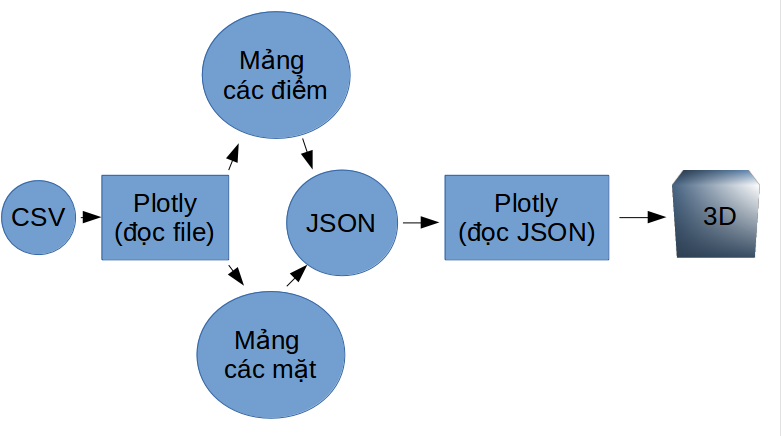
\includegraphics[totalheight=7cm]{Images/app_show3d.png}
    \caption{Luồng xử lý việc hiển thị mô hình 3D bằng Plotly}
    \label{skip_conn}
\end{figure}

\section{Các chức năng và kết quả hiển thị của ứng dụng}
Về phần hiển thị, trang web được xây dựng khá đơn giản nhưng đảm bảo được những thông tin cần thiết của kết quả phân đoạn một lá gan.
\subsection{Trang giới thiệu}
Trang này chỉ đơn giản là giới thiệu về chức năng của website.
\begin{figure}[h]
\centering
    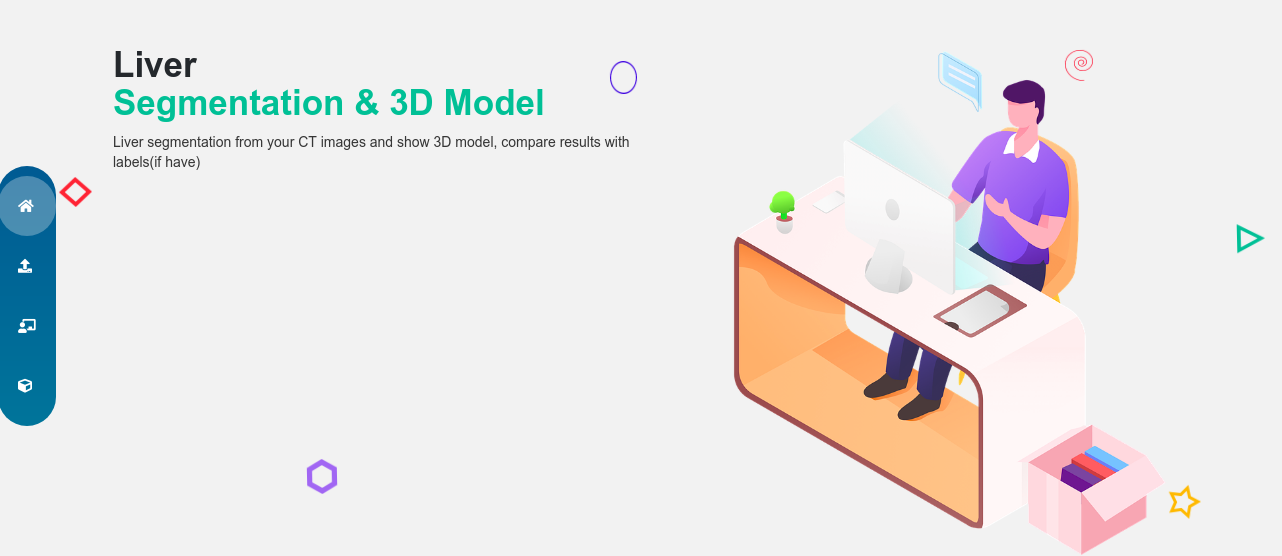
\includegraphics[totalheight=7cm]{Images/app_intro.png}
    \caption{Giao diện trang giới thiệu ứng dụng}
    \label{skip_conn}
\end{figure}
\subsection{Trang upload dữ liệu}
Trang này cho phép người dùng upload dữ liệu lên. Dữ liệu là tập scan có định dạng raw/mhd được nén trực tiếp ở dạng zip. Sau khi upload thì đợi kết quả trả về (chạy trên máy local mất khoảng 30 phút). Nếu dữ liệu có thêm nhãn thì kết quả trả về có dạng để so sánh. Kết quả sẽ được hiển thị ở trang tiếp theo.
\begin{figure}[h]
\centering
    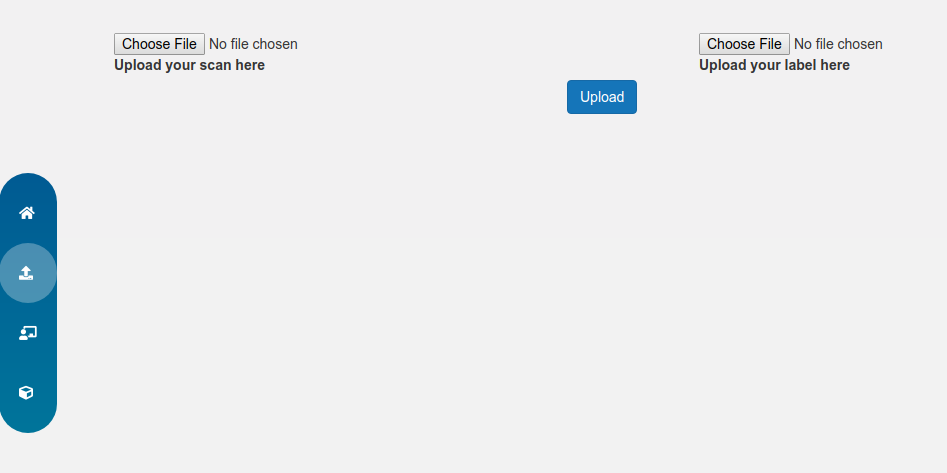
\includegraphics[totalheight=7cm]{Images/app_upload.png}
    \caption{Giao diện trang upload dữ liệu}
    \label{skip_conn}
\end{figure}
\subsection{Trang hiển thị kết quả phân đoạn}
Như đã nêu trên, nếu dữ liệu upload chỉ có scan, thì trang này hiển thị 3 mục như sau:
\begin{itemize}
    \item Ảnh scan(ảnh gốc lúc upload).
    \item Ảnh phân đoạn gan.
    \item Ảnh phân đoạn dán lên scan tương ứng.
\end{itemize}

\begin{figure}[h]
\centering
    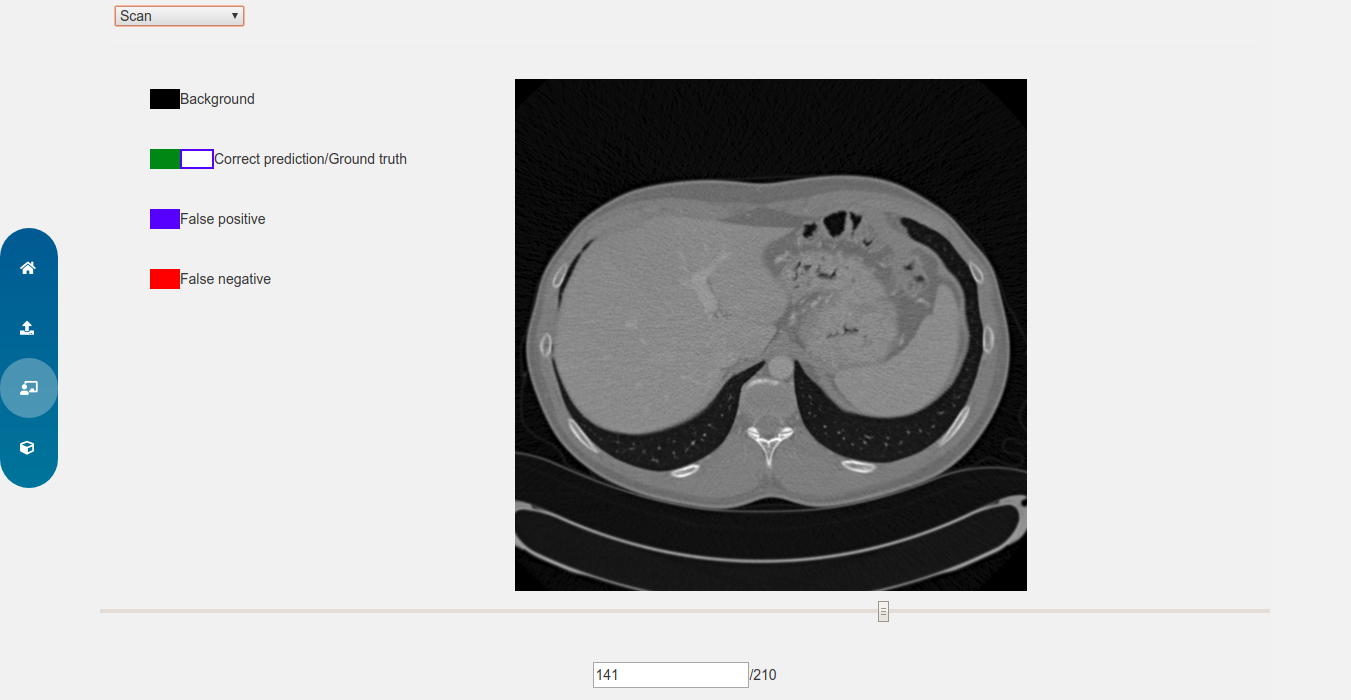
\includegraphics[totalheight=7cm]{Images/app_scan.png}
    \caption{Hiển thị ảnh scan}
    \label{skip_conn}
\end{figure}
\begin{figure}[h]
\centering
    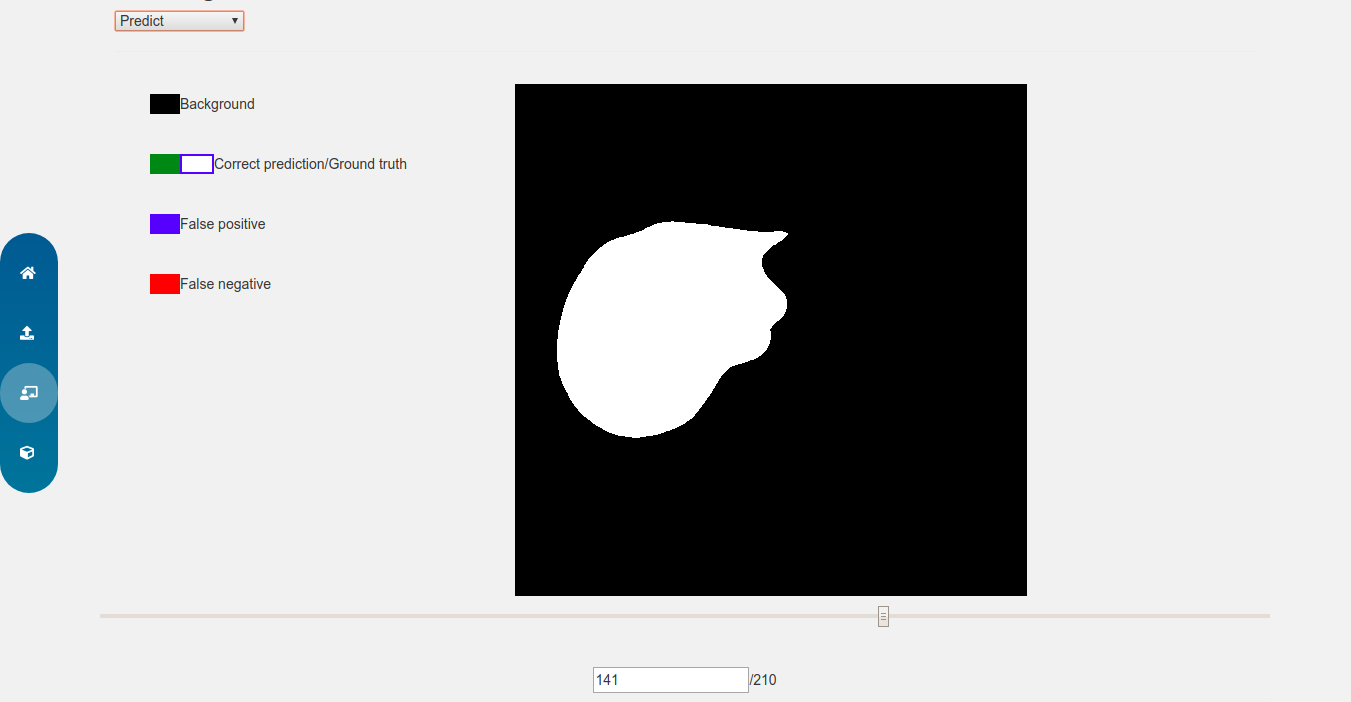
\includegraphics[totalheight=7cm]{Images/app_label.png}
    \caption{Hiển thị ảnh phân đoạn khi không có nhãn}
    \label{skip_conn}
\end{figure}
\begin{figure}[h]
\centering
    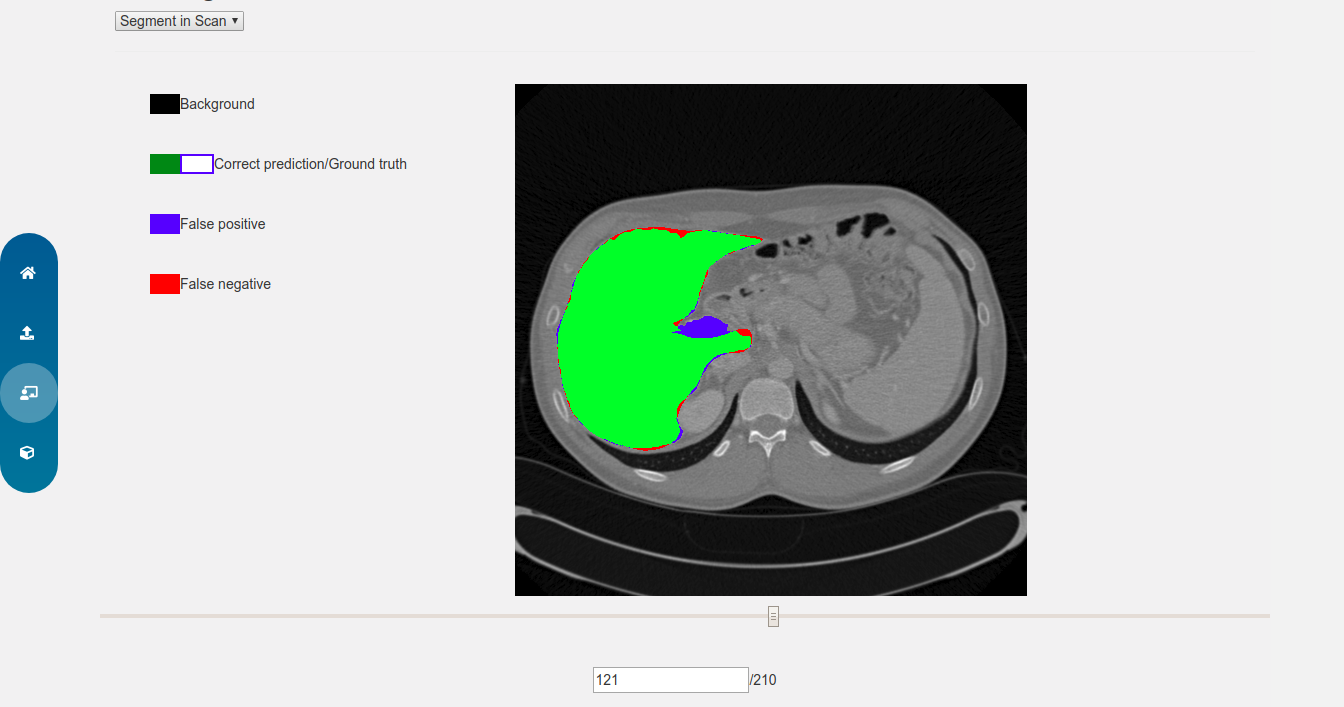
\includegraphics[totalheight=7cm]{Images/app_overlap_1.png}
    \caption{Hiển thị ảnh phân đoạn dán lên scan}
    \label{skip_conn}
\end{figure}
Nếu tập dữ liệu có thêm nhãn thì kết quả hiển thị có ảnh scan giống với mục trên, các ảnh còn lại sẽ là kết quả để so sánh với nhãn.
\begin{figure}[h]
\centering
    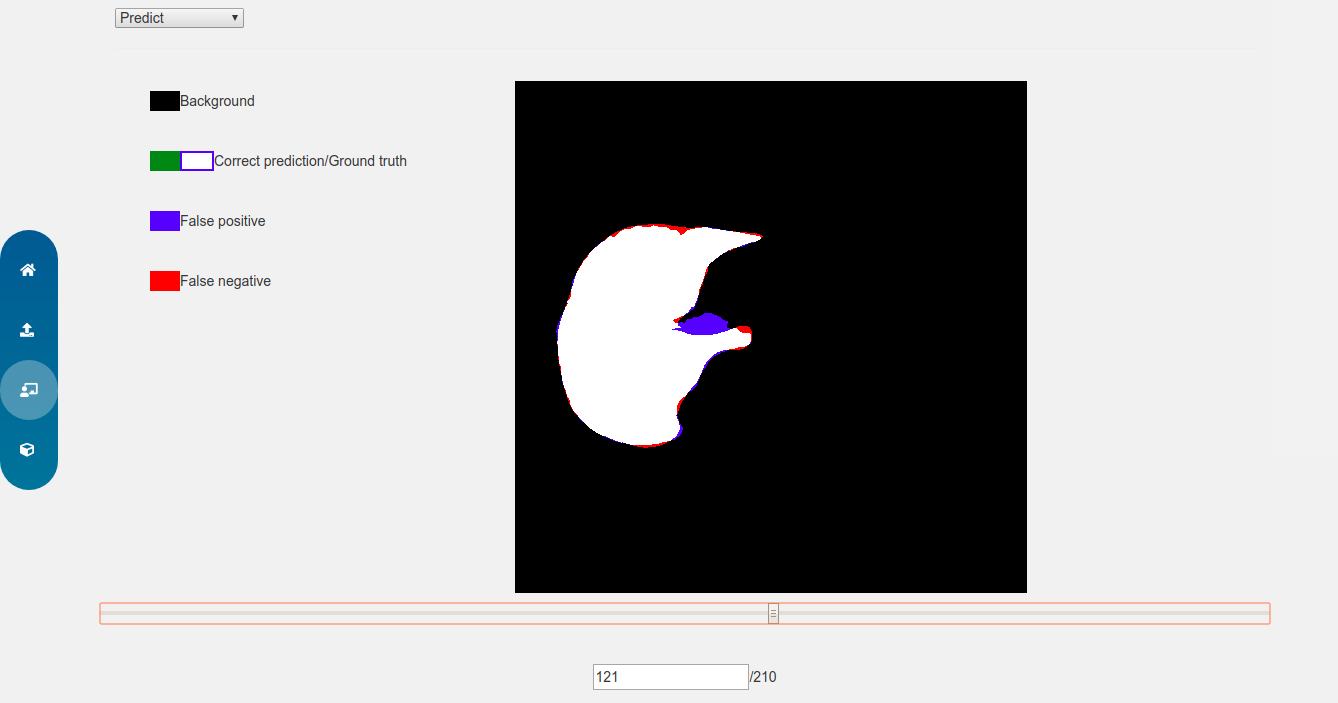
\includegraphics[totalheight=7cm]{Images/app_showscanompare.png}
    \caption{Hiển thị ảnh phân đoạn so sánh với nhãn}
    \label{skip_conn}
\end{figure}
\begin{figure}[h]
\centering
    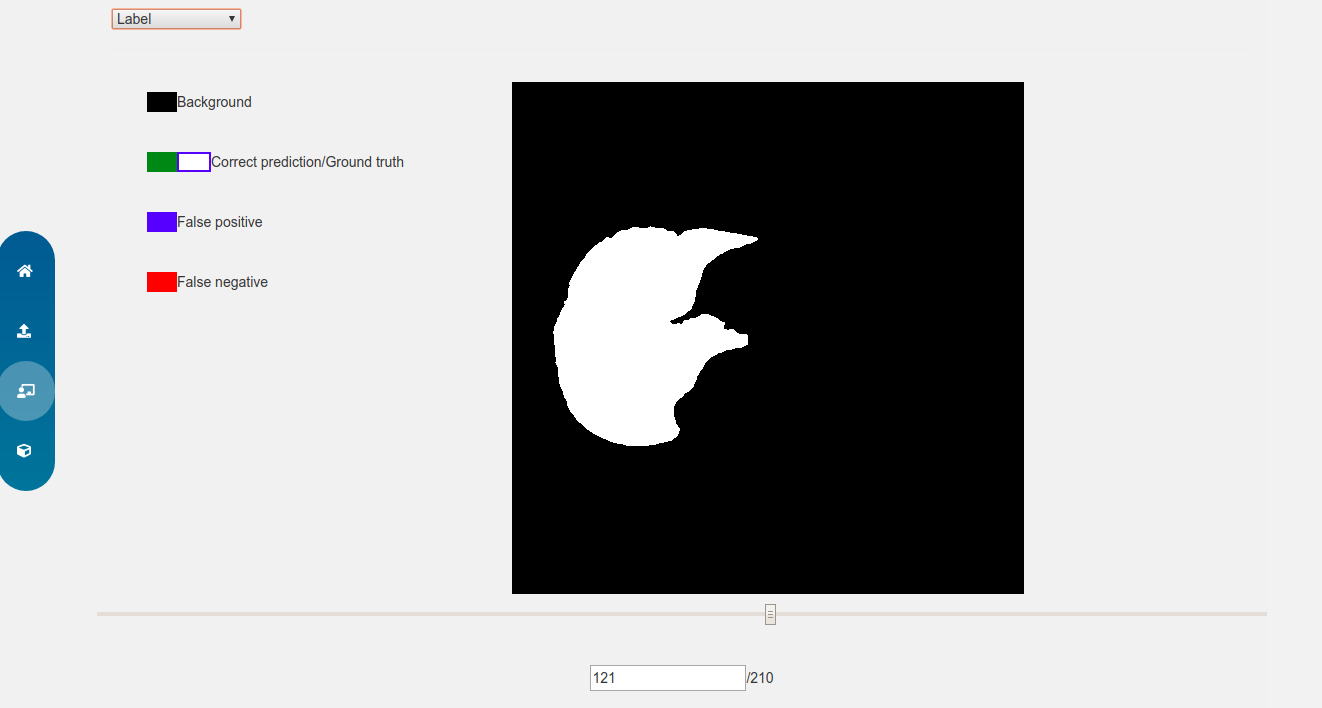
\includegraphics[totalheight=7cm]{Images/app_labelreal.png}
    \caption{Hiển thị ảnh nhãn}
    \label{skip_conn}
\end{figure}
\begin{figure}[h]
\centering
    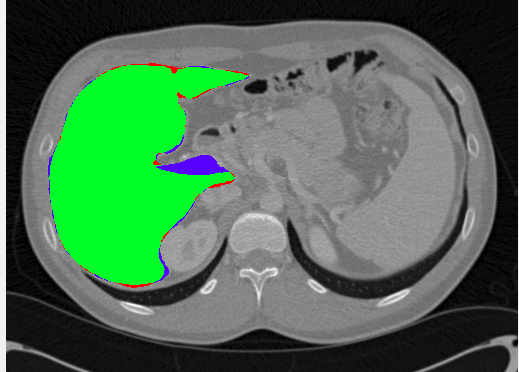
\includegraphics[totalheight=7cm]{Images/app_overlap_2.png}
    \caption{Hiển thị ảnh phân đoạn so sánh với nhãn dán lên scan}
    \label{skip_conn}
\end{figure}

\subsection{Trang hiển thị mô hình 3D}
Trang này hiển thị mô hình 3D bằng cách dùng thư viện plotly.js đọc file csv được tạo ra trong Django server đồng thời hiển thị thể tích của gan. Người dùng có thể dùng chuột để xoay, thu nhỏ, phóng to để xem chi tiết mô hình.
\begin{figure}[h]
\centering
    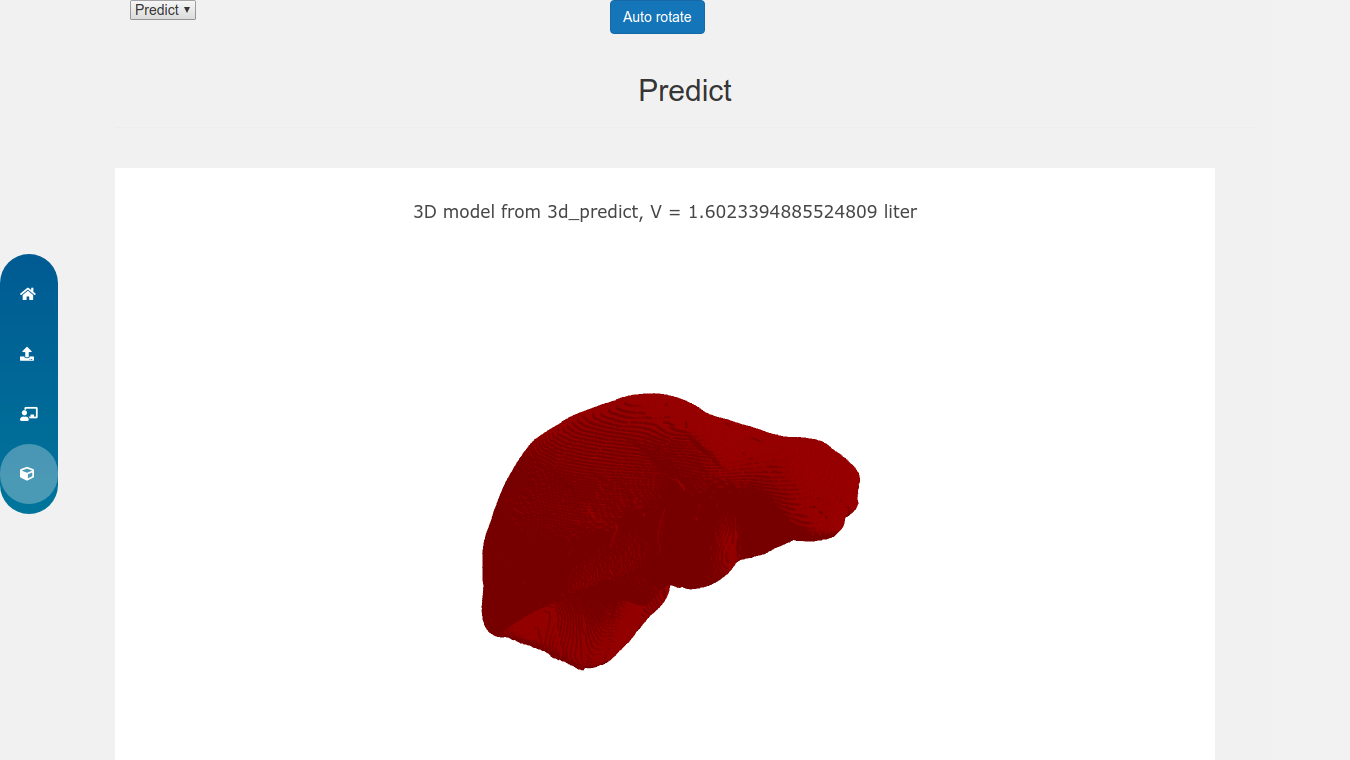
\includegraphics[totalheight=7cm]{Images/app_3dpredict.png}
    \caption{Hiển thị mô hình 3D dự đoán kèm thể tích}
    \label{skip_conn}
\end{figure}
\begin{figure}[h]
\centering
    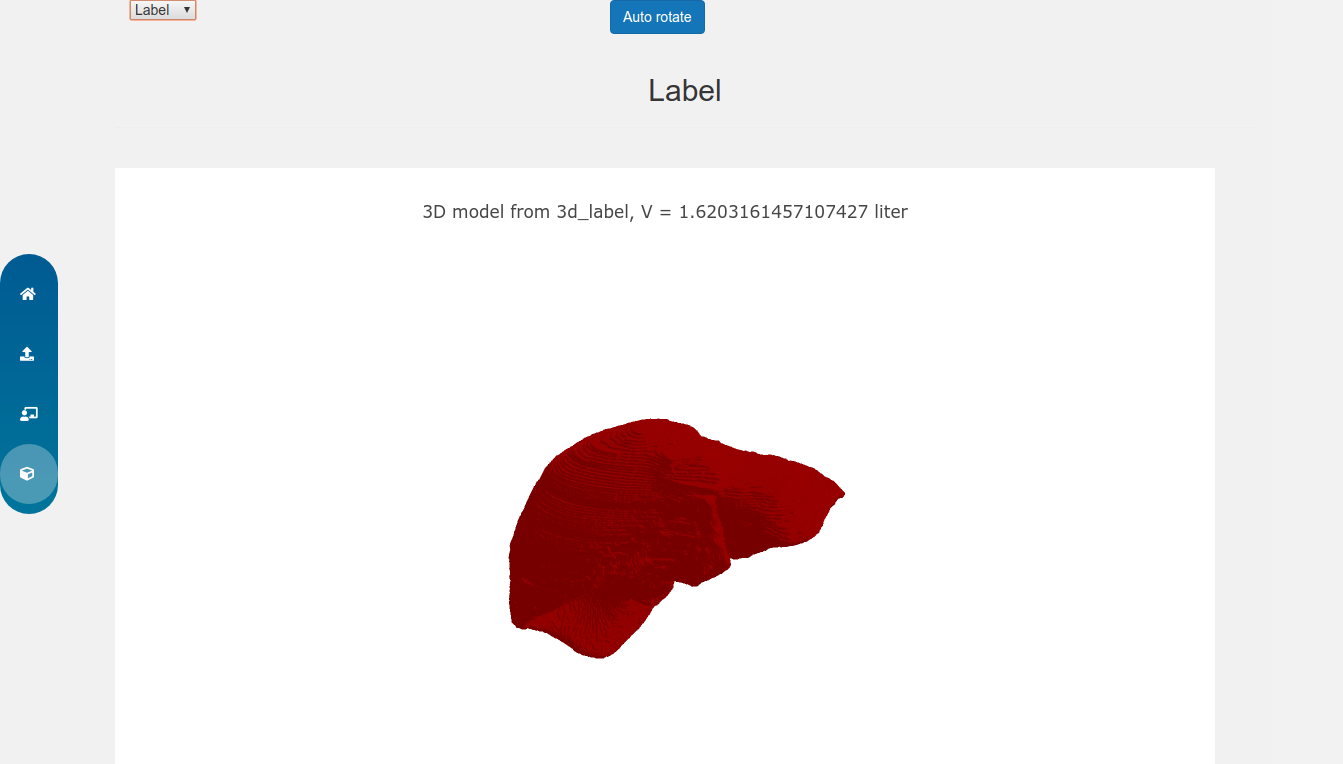
\includegraphics[totalheight=7cm]{Images/app_3dlabel.png}
    \caption{Hiển thị mô hình 3D của nhãn kèm thể tích}
    \label{skip_conn}
\end{figure}

Ta có thể click vào nút ``Auto rotate`` để lá gan xoay tự động. Một mô hình sẽ có khoảng hai trăm nghìn điểm và bốn trăm nghìn mặt nên chức năng tự động xoay khá chậm.
\section{Ưu nhược điểm của ứng dụng}
Ưu điểm:\\
\begin{itemize}
    \item Các thành phần được xây dựng riêng biệt với nhau nên dễ dàng sửa đổi và phát triển.
    \item Mô hình 3D dễ dàng điều chỉnh để xem chi tiết lá gan.
\end{itemize}
Nhược điểm:\\
\begin{itemize}
    \item Chưa có bảo mật.
    \item Giao diện còn khá đơn giản.
\end{itemize}



\chapter{Tổng kết}
% \section{Luồng xử lý dữ liệu hoàn chỉnh}
\section{Kết quả đạt được}
Với nỗ lực của các thành viên trong nhóm, đề tài đã đạt được những kết quả khả quan:
\begin{itemize}
    \item Phân đoạn gan: Đề tài đã xây dựng thành công một mô hình phân đoạn gan với độ chính xác rất cao, sẽ là công cụ hỗ trợ rất tốt cho việc xem ảnh chụp CT và chuẩn đoán các bệnh trên gan của các bác sĩ, đồng thời làm tiền đề để xây dựng mô hình phát hiện các bất thường trong lá gan từ ảnh CT.
    \item Các giải thuật tiền, hậu xử lý dữ liệu: Đề tài cũng cung cấp được các giải thuật về tiền và hậu xử lý dữ liệu khi huấn luyện. Tiền xử lý giúp việc huấn luyện thuận lợi và hậu xử lý giúp cho kết quả hiển thị được mượt mà hơn. Các giải thuật này cũng góp phần đáng kể trong việc tăng độ chính xác cho toàn mô hình. Đồng thời các đề tài khác cũng có thể áp dụng với một vài chỉnh sửa nhỏ tùy vào tập dữ liệu.
    \item Làm giàu dữ liệu: Đề tài cung cấp các giải thuật làm giàu bộ dữ liệu ảnh y khoa, làm cho mô hình dự đoán chính xác hơn, tránh overfitting. Các tập dữ liệu có nhãn hiếm hoi của những đề tài khác có thể áp dụng được những giải thuật này hoặc dựa vào đó để phát triển thêm các phương án làm giàu khác tùy thích, từ đó một phần giải quyết vấn đề khan hiếm dữ liệu có nhãn trong lĩnh vực học sâu.
    \item Đánh giá trên nhiều tập dữ liệu: Đề tài này sử dụng cả 3 tập dữ liệu có nhãn phổ biến nhất về lá gan từ trước đến nay để đánh giá độ chính xác của mô hình mà nhóm xây dựng đó là 3Dircadb, SLIVER07 và LITS2017. Trong đó tập 3Dircadb đạt độ chính xác gần 99\% với độ đo ``Dice per case``, tập SLIVER07 xếp hạng tối thiểu là thứ 16 (kết quả này cho mô hình trước đó, sau này không cho submit vì không có paper công khai) với điểm số trung bình là 79.89 trên ``SLIVER07 Grand Challenge 2007`` và tập LITS2017 đạt top 5 tại ``Liver Tumor Segmentation Challenge 2017``. Đây đều là những kết quả đạt được khá ấn tượng.
    \item Xây dựng ứng dụng hiển thị: Cuối cùng, đề trực quan hóa kết quả đạt được, nhóm đã xây dựng được một ứng dụng cho phép đăng tải dữ liệu ảnh CT và nhận kết quả phân đoạn đồng thời hiển thị mô hình 3D và tính thể tích gan tương ứng cho dữ liệu đó. Tất cả các kết quả đều được hiển thị trên giao diện web - hiện nay là phương án tiếp cận phổ biến, dễ sử dụng, dễ tuỳ chỉnh và hiệu quả nhất cho các ứng dụng nhỏ.
\end{itemize}
\section{Hạn chế và hướng phát triển}
Tuy kết quả của đề tài này thực sự rất tốt với những yêu cầu đã đề ra ban đầu, nhưng vẫn còn một số hạn chế như sau:
\begin{itemize}
    \item Đề tài này cần kết hợp với những đề tài khác như phân đoạn mạch máu và dự đoán bất thường trong gan, khi đó mới đem lại ý nghĩa thực tiễn to lớn trong việc xem và chuẩn đoán các bệnh về gan của các bác sĩ, đồng thời giúp các bác sĩ ra quyết định trong việc cắt và ghép lá gan qua ảnh CT (điều này nhóm nhận ra qua buổi hướng dẫn của các bác sĩ tại Bệnh viện Đại học Y Dược).
    \item Ứng dụng xây dựng chỉ áp dụng cho tập dữ liệu có định dạng ảnh CT chuẩn có thể đọc được bằng thư viện SimpleItk như mhd|raw, nii, niiz.
\end{itemize}
Với những nhược điểm và những yêu cầu hiện ở thời điểm hiện tại, nhóm đề xuất một số hướng phát triển cho đề tài này.
\begin{itemize}
    \item Kết hợp với mô hình phân đoạn mạch máu trong gan thành một mô hình phân đoạn cả gan lẫn mạch máu hoàn chỉnh (vì mạch máu nằm trong gan nên kết hợp hai mô hình một lúc sẽ đem lại kết quả tốt hơn việc chạy riêng biệt hai mô hình và lấy 2 kết quả ghép lại).
    \item Xây dựng ứng dụng hiển thị kết quả phân đoạn và mô hình 3D cho hệ thống gan - mạch máu hoàn chỉnh.
    \item Xây dựng mô hình tương tự để phân đoạn những cơ quan khác trong cơ thể từ ảnh CT.
\end{itemize}




\bibliography{refs}{}
\bibliographystyle{plainurl}
%-	Danh mục TL tham khảo
%-	Phụ lục (nếu có)

\end{document}
